% cSpell:language es,en
\documentclass[12pt,a4paper,oneside]{book}


% PREÁMBULO: Todos los paquetes y configuraciones
\usepackage{booktabs}
\usepackage{array}
\usepackage{longtable}
\usepackage{multirow}
\usepackage{tikz}
\usetikzlibrary{positioning, shapes.geometric, arrows.meta, babel, shadows}



% Idioma y codificación
\usepackage[utf8]{inputenc}
\usepackage[spanish,es-tabla]{babel}
\usepackage[T1]{fontenc}
\usepackage{lmodern}

% Geometría y márgenes
\usepackage[top=2.5cm, bottom=2.5cm, left=3cm, right=2.5cm]{geometry}
\usepackage{setspace}
\onehalfspacing

% Bibliografía
\usepackage{csquotes}
\usepackage[backend=biber,style=ieee,sorting=none]{biblatex}
\addbibresource{referencias.bib}

% Gráficos y figuras
\usepackage{graphicx}
\graphicspath{{media/}{figures/}{imagenes/}}
\usepackage{float}
\usepackage{caption}
\usepackage{subcaption}

% Tablas
\usepackage{booktabs}
\usepackage{multirow}
\usepackage{array}
\usepackage{longtable}
\usepackage{tabularx}

% Matemáticas
\usepackage{amsmath}
\usepackage{amssymb}
\usepackage{amsthm}

% Hipervínculos
\usepackage[hidelinks]{hyperref}
\usepackage{url}
\urlstyle{same}

% Listas
\usepackage{enumitem}
\setlist[itemize]{leftmargin=*}
\setlist[enumerate]{leftmargin=*}
\setlist[description]{leftmargin=0cm,style=nextline}

% Encabezados
\usepackage{fancyhdr}
\pagestyle{fancy}
\fancyhf{}
\fancyhead[R]{\thepage}
\fancyhead[L]{\nouppercase{\leftmark}}
\renewcommand{\headrulewidth}{0.4pt}
\fancypagestyle{plain}{%
    \fancyhf{}
    \fancyfoot[C]{\thepage}
    \renewcommand{\headrulewidth}{0pt}
}

% Código fuente
\usepackage{listings}
\usepackage{xcolor}

% Definir lenguaje JSON para listings
\lstdefinelanguage{json}{
    basicstyle=\small\ttfamily,
    numbers=left,
    numberstyle=\tiny\color{codegray},
    stepnumber=1,
    numbersep=8pt,
    showstringspaces=false,
    breaklines=true,
    frame=single,
    backgroundcolor=\color{backcolour},
    string=[s]{"}{"},
    stringstyle=\color{codepurple},
    comment=[l]{//},
    morecomment=[s]{/*}{*/},
    commentstyle=\color{codegreen},
    morestring=[b]',
    morestring=[b]"
}

\definecolor{codegreen}{rgb}{0,0.6,0}
\definecolor{codegray}{rgb}{0.5,0.5,0.5}
\definecolor{codepurple}{rgb}{0.58,0,0.82}
\definecolor{backcolour}{rgb}{0.95,0.95,0.92}

\lstdefinestyle{mystyle}{
    backgroundcolor=\color{backcolour},   
    commentstyle=\color{codegreen},
    keywordstyle=\color{magenta},
    numberstyle=\tiny\color{codegray},
    stringstyle=\color{codepurple},
    basicstyle=\ttfamily\footnotesize,
    breakatwhitespace=false,         
    breaklines=true,                 
    captionpos=b,                    
    keepspaces=true,                 
    numbers=left,                    
    numbersep=5pt,                  
    showspaces=false,                
    showstringspaces=false,
    showtabs=false,                  
    tabsize=2
}
\lstset{style=mystyle}

% Formato de capítulos
\usepackage{titlesec}
\usepackage{titlesec}

% Solo modifica el índice, no los títulos
\usepackage{titletoc}
\titlecontents{chapter}
  [0em]                           % margen izquierdo
  {\bfseries}                     % formato
  {Capítulo \thecontentslabel. }  % antes del título
  {}                              % sin número
  {\titlerule*[1pc]{.}\contentspage}  % puntos y número de página

% Capítulos: tamaño 14pt
\titleformat{\chapter}[hang]
{\normalfont\fontsize{14}{16}\bfseries\selectfont}{\chaptertitlename\ \thechapter.}{1em}{}

\titlespacing*{\chapter}{0pt}{0.35\textheight}{40pt}

% Capítulos sin número (Introducción, Conclusiones): tamaño 14pt
\titleformat{name=\chapter,numberless}[hang]
{\normalfont\fontsize{14}{16}\bfseries\selectfont}{}{0pt}{}

\titlespacing*{name=\chapter,numberless}{0pt}{0.35\textheight}{40pt}

% Comando especial para páginas sin espacio arriba
\newcommand{\chapternospacetop}[1]{%
  \begingroup
  \titlespacing*{name=\chapter,numberless}{0pt}{0pt}{20pt}%
  \chapter*{#1}%
  \endgroup
}

% Secciones (1.1, 1.2): tamaño 13pt
\titleformat{\section}
{\normalfont\fontsize{13}{15}\bfseries\selectfont}{\thesection}{1em}{}

% Subsecciones (1.1.1, 1.1.2): tamaño 12pt
\titleformat{\subsection}
{\normalfont\fontsize{12}{14}\bfseries\selectfont}{\thesubsection}{1em}{}

% Subsubsecciones (1.1.1.1): tamaño 12pt
\titleformat{\subsubsection}
{\normalfont\fontsize{12}{14}\bfseries\selectfont}{\thesubsubsection}{1em}{}

% Referencias cruzadas
\usepackage{cleveref}
\crefname{figure}{Figura}{Figuras}
\crefname{table}{Tabla}{Tablas}
\crefname{equation}{Ecuación}{Ecuaciones}
\crefname{chapter}{Capítulo}{Capítulos}
\crefname{section}{Sección}{Secciones}
\crefname{appendix}{Apéndice}{Apéndices}

% Espaciado
\setlength{\parskip}{0.5em}
\setlength{\parindent}{0pt}

% Comandos personalizados
\newcommand{\universidad}{Pontificia Universidad Católica del Perú}
\newcommand{\facultad}{Facultad de Ciencias e Ingeniería}
\newcommand{\especialidad}{Ingeniería de las Telecomunicaciones}
\newcommand{\autor}{Juan Alfonso Chapoñan Espinoza}
\newcommand{\asesor}{Oscar Antonio Díaz Barriga}
\newcommand{\ciudad}{Lima}
\newcommand{\anio}{2025}

% PDF metadata
\hypersetup{
    pdftitle={Plataforma Web y Móvil con IA para Delivery Urbano},
    pdfauthor={Juan Alfonso Chapoñan Espinoza},
    pdfsubject={Tesis de Ingeniería de Telecomunicaciones},
    pdfkeywords={IoT, IA, Delivery, Logística, Computer Vision},
}

% Idioma
\addto\captionsspanish{
    \renewcommand{\listtablename}{ÍNDICE DE TABLAS}
    \renewcommand{\listfigurename}{ÍNICE DE FIGURAS}
    \renewcommand{\tablename}{Tabla}
    \renewcommand{\figurename}{Figura}
    \renewcommand{\contentsname}{ÍNDICE}
}


% INFORMACIÓN DEL DOCUMENTO

\title{Diseño e implementación de una plataforma web-móvil para gestión logística en PyMEs con medición automática de dimensiones de paquetes mediante inteligencia artificial}
\author{Juan Alfonso Chapoñan Espinoza}
\date{Lima, agosto, 2025}


% INICIO DEL DOCUMENTO

\begin{document}

% ------------------------------------------------------------------
% PÁGINAS PRELIMINARES SIN NUMERACIÓN (no se cuentan)
% ------------------------------------------------------------------
\pagenumbering{gobble}  % Desactiva completamente la numeración

% ==================================================================
% PORTADA
% ==================================================================

\begin{titlepage}
    \centering
    \vspace*{1cm}
    
    {\Large\textbf{\universidad}}\\[0.5cm]
    {\Large\textbf{\facultad}}\\[1.5cm]
    
    % Logo PUCP (descomentar y ajustar ruta cuando tengas la imagen)
    % 
\includegraphics[width=0.25\textwidth]{logo_pucp.png}\\[1.5cm]
    
    \vspace{1cm}
    
    {\large\textbf{DISEÑO E IMPLEMENTACIÓN DE UNA PLATAFORMA WEB Y APLICACIÓN MÓVIL CON PROCESAMIENTO DE IMÁGENES CON INTELIGENCIA ARTIFICIAL MULTIMODAL EN LA NUBE PARA LA IDENTIFICACIÓN DE PAGOS, ESTIMACIÓN DE DIMENSIONES Y OPTIMIZACIÓN LOGÍSTICA EN SERVICIOS DE DELIVERY URBANO EN LIMA}}\\[2.5cm]
    
    {\large Tesis para obtener el título profesional de}\\[0.3cm]
    {\large\textbf{Ingeniero de las Telecomunicaciones}}\\[2.5cm]
    
    {\large \textbf{Que presenta:}}\\[0.3cm]
    {\large \autor}\\[2cm]
    
    {\large \textbf{Asesor:}}\\[0.3cm]
    {\large \asesor}\\[2cm]
    
    \vfill
    
    {\large \ciudad, junio, \anio}
\end{titlepage}
\cleardoublepage
\titlespacing*{name=\chapter,numberless}{0pt}{0pt}{20pt}

\chapter*{INFORME DE SIMILITUD}
%\addcontentsline{toc}{chapter}{Informe de Similitud}

\vspace{1cm}

Yo, \textbf{OSCAR ANTONIO DÍAZ BARRIGA}, docente de la Facultad de \textbf{CIENCIAS E INGENIERÍA} de la Pontificia Universidad Católica del Perú, asesor de la tesis titulada \textbf{PLATAFORMA WEB Y MÓVIL CON PROCESAMIENTO DE IMÁGENES EN LA NUBE E INTELIGENCIA ARTIFICIAL PARA LA IDENTIFICACIÓN DE PAGOS, ESTIMACIÓN DE DIMENSIONES Y OPTIMIZACIÓN LOGÍSTICA EN SERVICIOS DE DELIVERY URBANO EN LIMA}, del autor \textbf{JUAN ALFONSO CHAPOÑAN ESPINOZA}, dejo constancia de lo siguiente:

\begin{itemize}
    \item El mencionado documento tiene un índice de puntuación de similitud de \textbf{[\#\#]\%}. Así lo consigna el reporte de similitud emitido por el software Turnitin el \textbf{[DD/MM/AAAA]}.
    
    \item He revisado con detalle dicho reporte y la Tesis, y no se advierte indicios de plagio.
    
    \item Las citas a otros autores y sus respectivas referencias cumplen con las pautas académicas.
\end{itemize}

\vspace{1.5cm}

\textbf{Lugar y fecha:} San Miguel, [DD] de [MES] de [AAAA].

\vspace{2cm}

\begin{table}[H]
\centering
\begin{tabular}{|p{7cm}|p{7cm}|}
\hline
Apellidos y nombres del asesor: & \\
\textbf{DÍAZ BARRIGA, OSCAR ANTONIO} & \\
\hline
DNI: \textbf{71477000} & Firma \\
\hline
ORCID: 0000-0002-9930-5984 & \\
\hline
\end{tabular}
\end{table}

\cleardoublepage

% ------------------------------------------------------------------
% INICIA NUMERACIÓN ROMANA DESDE i
% ------------------------------------------------------------------
\frontmatter
\pagestyle{plain}  % Activa numeración romana

\chapter*{DEDICATORIA}
\addcontentsline{toc}{chapter}{DEDICATORIA}
A mis padres.

\cleardoublepage

\chapter*{AGRADECIMIENTOS}
\addcontentsline{toc}{chapter}{AGRADECIMIENTOS}
[Por completar]
\cleardoublepage

\chapter*{RESUMEN}
\addcontentsline{toc}{chapter}{RESUMEN}
[Por completar]
\cleardoublepage

\tableofcontents
\addcontentsline{toc}{chapter}{\contentsname}
\cleardoublepage

\listoftables
\addcontentsline{toc}{chapter}{\listtablename}
\cleardoublepage

\listoffigures
\addcontentsline{toc}{chapter}{\listfigurename}

\cleardoublepage

\chapter*{GLORASIO}
\addcontentsline{toc}{chapter}{GLOSARIO}
[Por completar]
\cleardoublepage

% ------------------------------------------------------------------
% CONTENIDO PRINCIPAL
% ------------------------------------------------------------------
\mainmatter  

\chapter*{INTRODUCCIÓN}
\addcontentsline{toc}{chapter}{INTRODUCCIÓN}
[Por completar]

% cSpell:language es,en
% ==================================================================
% CAPÍTULO 1: PRESENTACIÓN DEL PROBLEMA DE INGENIERÍA
% ==================================================================

\chapter{Presentación del problema de ingeniería}

La transformación digital en el sector logístico demanda soluciones innovadoras que aprovechen tecnologías emergentes para resolver desafíos operacionales críticos. Esta investigación aborda la problemática de la inexactitud en la determinación de dimensiones de paquetes en la industria de \textit{delivery}, factor que genera ineficiencias significativas en la planificación de rutas y utilización de capacidad vehicular. Mediante la convergencia de aplicaciones IoT, procesamiento de imágenes con inteligencia artificial y arquitecturas distribuidas en la nube, se propone una solución integral que mejora la precisión operacional y democratiza el acceso a tecnologías sofisticadas para empresas de diferentes escalas.

% ------------------------------------------------------------------
\section{Identificación temática y motivación personal}
% ------------------------------------------------------------------

\subsection{Área de especialización en telecomunicaciones}

\subsubsection{Aplicaciones IoT (\textit{Internet of Things})}

Las aplicaciones IoT constituyen un ecosistema tecnológico integral que integra inteligencia artificial, redes de comunicación y automatización para crear una infraestructura de conectividad ubicua entre objetos físicos y sistemas digitales \cite{Liu2013}. Se define como la implementación de una arquitectura de cinco capas interconectadas:

\begin{table}[H]
\centering
\caption{Arquitectura IoT \cite{Zhou2022}.}
\label{tab:arquitectura_iot}
\begin{tabular}{@{}ll@{}}
\toprule
\textbf{Capa} & \textbf{Descripción} \\
\midrule
Percepción & Sensores y dispositivos de captura \\
Red & Protocolos de comunicación y transmisión \\
Middleware & Procesamiento y almacenamiento de datos \\
Aplicación & Servicios e interfaces de usuario \\
Negocio & Análisis y toma de decisiones \\
\bottomrule
\end{tabular}
\end{table}

\subsubsection{Servicios de Telecomunicaciones para Logística}

Los servicios de telecomunicaciones para logística se definen como el conjunto de tecnologías y protocolos de comunicación que operan principalmente en la capa de red del ecosistema IoT, actuando como puente crítico entre la percepción de datos y su procesamiento funcional. Estos servicios garantizan la transmisión eficiente y segura de información tanto estática como móvil durante todas las fases del proceso logístico \cite{Zhou2022}.

\subsubsection{Convergencia Tecnológica}

La tesis desarrollada en esta investigación representa la convergencia de múltiples disciplinas dentro de la ingeniería de telecomunicaciones:

\begin{itemize}
    \item \textbf{Arquitecturas Distribuidas en la Nube}: Para el procesamiento remoto y almacenamiento escalable
    \item \textbf{Inteligencia Artificial}: Específicamente visión por computadora para el procesamiento automatizado de imágenes
\end{itemize}

Esta integración tecnológica permite abordar desafíos reales del sector logístico mediante soluciones que aprovechan las capacidades de procesamiento remoto, almacenamiento distribuido y comunicaciones continuas, características fundamentales de los sistemas modernos de telecomunicaciones en el contexto de la transformación digital.

% ------------------------------------------------------------------
\subsection{Relación con los estudios realizados}
% ------------------------------------------------------------------

La presente investigación se fundamenta en una progresión curricular especializada que abarca desde los fundamentos del desarrollo web hasta la implementación de soluciones IoT avanzadas, estableciendo una relación directa y sistemática con tres cursos clave que proporcionan las competencias técnicas necesarias.

\subsubsection{TEL131 Ingeniería Web para Telecomunicaciones}

Este curso proporciona la base tecnológica para desarrollar la capa de aplicación e interfaces de gestión en soluciones de logística inteligente. Se abordan fundamentos de programación, desarrollo web con conexión a bases de datos, y modelado relacional con SQL, aplicables en \textit{dashboards} para monitoreo en tiempo real, interfaces de control y manejo de datos IoT.

\subsubsection{TEL137 Gestión de Servicios de TICs}

Este curso se enfoca en la gestión de servicios dentro del ecosistema IoT, brindando competencias para desarrollar infraestructuras seguras, escalables y robustas. A través de \textit{frameworks} modernos y servicios web, se construyen sistemas capaces de optimizar rutas y asignar recursos inteligentemente.

\subsubsection{1TEL05 Servicios y Aplicaciones para IoT}

Este curso se centra en la construcción de la capa de aplicación IoT y su integración con la nube, facilitando el desarrollo de soluciones logísticas orientadas al usuario final. Se abordan competencias en aplicaciones móviles conectadas a servicios SaaS, útiles para rastreo de productos y alertas inteligentes.

% ------------------------------------------------------------------
\subsection{Motivación personal y experiencia profesional}
% ------------------------------------------------------------------

La motivación personal para abordar esta problemática combina una vocación por la automatización de procesos con un interés social en mejorar la eficiencia empresarial. La experiencia profesional durante la carrera, desde almacenero hasta asistente logístico, brindó una comprensión directa de los desafíos operacionales, destacando la importancia del cumplimiento de tiempos en cada etapa del proceso logístico.

% ------------------------------------------------------------------
\section{Descripción y características del problema}
% ------------------------------------------------------------------

\subsection{Contexto del problema en la industria de \textit{delivery}}

La industria de servicios de \textit{delivery} y logística de última milla ha experimentado un crecimiento exponencial en los últimos años, impulsada por el auge del comercio electrónico y los cambios en los hábitos de consumo de la población \cite{RedacciponTLW2025}. 

\begin{table}[H]
\centering
\caption{Proyecciones del Mercado de delivery en Perú.}
\label{tab:proyecciones_delivery}
\begin{tabular}{@{}lcc@{}}
\toprule
\textbf{Año} & \textbf{Crecimiento (\%)} & \textbf{Ingresos (millones USD)} \\
\midrule
2024 & --- & 2,500 \\
2029 & 11.03 & 2,951 \\
\bottomrule
\end{tabular}
\end{table}

Uno de los principales desafíos que enfrentan las empresas de \textit{delivery} es obtener información precisa sobre las dimensiones y características de los paquetes que deben recoger y entregar.

\subsection{Desafío técnico desde la perspectiva de telecomunicaciones}

Desde la perspectiva de la ingeniería de telecomunicaciones, el problema central radica en la necesidad de desarrollar un sistema distribuido que permita el procesamiento automatizado de imágenes capturadas por dispositivos móviles para la determinación precisa de dimensiones de paquetes.

\subsection{Características específicas del problema}

El problema presenta características específicas que lo hacen particularmente complejo desde el punto de vista técnico y operacional:

\begin{itemize}
    \item Gran variabilidad en dimensiones, formas y características físicas de los paquetes
    \item Limitación de capacidad de los motorizados
    \item Necesidad de confiabilidad en los procesos de verificación
    \item Requisito de escalabilidad del sistema
\end{itemize}

% ------------------------------------------------------------------
\section{Importancia del problema y su solución}
% ------------------------------------------------------------------

\subsection{Perspectiva técnica}

Resolver este problema es clave por el uso de tecnologías emergentes que transforman telecomunicaciones y computación distribuida. El procesamiento en la nube ha madurado para realizar análisis complejos de imágenes sin necesidad de ejecución local en dispositivos \cite{Xu2012,Wang2012}.

\subsection{Perspectiva económica y financiera}

La automatización en medición de paquetes mejora rentabilidad y competitividad logística, generando ahorros significativos y optimizando recursos de transporte \cite{Krysiska2024}.

\begin{figure}[H]
    \centering
    % \includegraphics[width=0.8\textwidth]{gastos_tecnologia.png}
    \caption{Gasto en tecnologías de la información - América Latina.}
    \label{fig:gastos_tecnologia}
\end{figure}

\subsection{Perspectiva social y cultural}

Socialmente, la solución mejora la calidad de vida de trabajadores logísticos y usuarios finales. La automatización de tareas repetitivas permite enfocar recursos humanos en actividades de mayor valor, mejorando satisfacción laboral y desarrollo profesional.

\subsection{Perspectiva ambiental y de sostenibilidad}

Abordar este problema es clave para reducir emisiones de gases de efecto invernadero y usar recursos energéticos eficientemente. La optimización de rutas, basada en medidas precisas de paquetes, permite planificar trayectos más cortos, disminuyendo consumo de combustible y emisiones de CO₂.

\subsection{Perspectiva legal y reglamentaria}

En Perú, la medición automatizada de paquetes con IoT debe cumplir la Ley N.º 29733, que exige consentimiento previo, finalidad clara, calidad y seguridad en el tratamiento de datos \cite{EditoraPer2973}.

\subsection{Perspectiva ética}

La automatización plantea dilemas éticos sobre responsabilidad social, equidad digital, sostenibilidad ambiental, privacidad de datos y rendición de cuentas. Esta visión ética integral asegura que la tecnología respete valores humanos y apoye un desarrollo sostenible.

% ------------------------------------------------------------------
\section{Impactos previstos y beneficiarios}
% ------------------------------------------------------------------

\subsection{Impactos operacionales}

La implementación tendrá impactos operacionales significativos, mejorando la eficiencia mediante tecnologías IoT, IA y visión artificial \cite{RedaccinTLW2024,Alharbi2023}.

\subsubsection{Reducción de tiempos de procesamiento}

La medición automatizada elimina procesos manuales, reduciendo el tiempo requerido para registrar, verificar y procesar solicitudes \cite{Xu2012}.

\subsubsection{Optimización de rutas de entrega}

Con datos precisos sobre dimensiones, los sistemas pueden planificar rutas más eficientes considerando capacidad de carga, tiempo y distancia.

\subsection{Impactos tecnológicos}

La implementación tendrá un impacto tecnológico significativo en telecomunicaciones e IoT, estableciendo nuevos paradigmas en procesamiento de imágenes para logística.

\subsection{Impactos económicos}

Los impactos económicos se reflejan desde la productividad individual hasta la competitividad sectorial, aprovechando procesamiento de imágenes con IA en la nube para optimizar entregas urbanas.

\subsection{Beneficiarios directos}

\subsubsection{Empresas de \textit{delivery} y logística}

Son los principales beneficiarios, mejorando eficiencia y rentabilidad gracias al procesamiento de imágenes con IA en la nube.

\subsubsection{Motorizados y personal operativo}

Mejoran productividad y condiciones laborales mediante rutas optimizadas que permiten más entregas en menos tiempo.

\subsubsection{Clientes emisores de paquetes}

Experimentan mayor fiabilidad y transparencia con rutas inteligentes que optimizan entregas y recojo.

\subsubsection{Destinatarios de entregas}

Reciben un servicio más rápido y predecible, cumpliendo estándares de \textit{quick commerce} en menos de 90 minutos.

\subsection{Beneficiarios indirectos}

\subsubsection{Sector de Telecomunicaciones}

Este sector verá un aumento en la demanda de servicios especializados y mejoras en infraestructura.

\subsubsection{Industria de Desarrollo de Software}

Se generarán nuevas oportunidades y mayor demanda de talento especializado en aplicaciones móviles, NoSQL y microservicios.

\subsubsection{Medio Ambiente y Sociedad}

La optimización de rutas reducirá emisiones de CO₂ y consumo de combustible, contribuyendo a un entorno urbano más saludable.

\subsubsection{Ecosistema de Innovación Tecnológica}

La solución fortalecerá la innovación al demostrar cómo tecnologías emergentes resuelven problemas reales.
% cSpell:language es,en
% ==================================================================
% CAPÍTULO 2: ESTADO DEL ARTE
% ==================================================================

\chapter{Estado del arte o de la cuestión, alternativas de solución al problema o desafío a resolver}

% ------------------------------------------------------------------
\section{Antecedentes de solución semejantes o similares al desafío de ingeniería}
% ------------------------------------------------------------------

\subsection{Sistemas de análisis visual con inteligencia artificial multimodal}

\subsubsection{Caso 1: GPT-4 Vision para análisis de objetos (OpenAI, Estados Unidos, 2023)}

GPT-4 Vision, lanzado en septiembre de 2023, representa el primer modelo de lenguaje de gran escala con capacidades multimodal nativas de OpenAI. El sistema demuestra capacidades avanzadas de interpretación visual con un 95\% de precisión en reconocimiento de objetos comunes y 78.5\% de efectividad en análisis de gráficos complejos según evaluaciones técnicas independientes \cite{ArticleRef255136}.

En términos de estimación dimensional, GPT-4V utiliza razonamiento contextual para comparar tamaños relativos entre objetos, empleando elementos conocidos como referencias de escala. Las evaluaciones técnicas reportan una precisión de $\pm$15--25\% de error en estimaciones dimensionales cuando se proporcionan referencias visuales adecuadas, mejorando a $\pm$10--20\% bajo condiciones de iluminación controlada \cite{Yu2024}.

\begin{figure}[H]
    \centering
    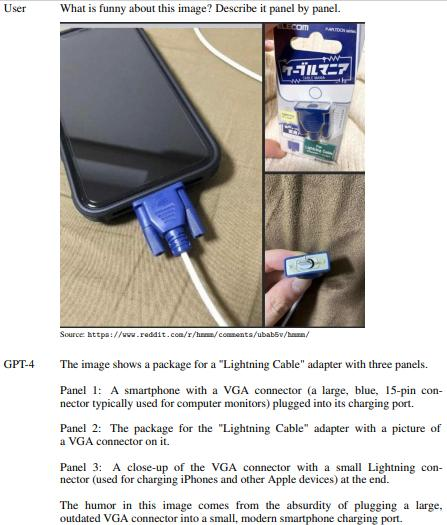
\includegraphics[width=0.9\textwidth]{gpt4_vision_example.png}
    \caption{Consulta a GPT-4 para análisis de múltiples imágenes. Fuente \cite{ArticleRef255134}}
    \label{fig:gpt4_vision}
\end{figure}

La arquitectura se basa en un \textit{transformer} multimodal que integra un codificador visual especializado con el modelo de lenguaje GPT-4, estimado en 1.76 trillones de parámetros. El sistema procesa imágenes de hasta 2048$\times$2048 píxeles en formatos JPEG, PNG, GIF y WebP, utilizando técnicas de atención cruzada para correlacionar información visual con conocimiento lingüístico \cite{ArticleRef255134}.

El modelo emplea un enfoque de \textit{vision-language understanding} que permite no solo identificar objetos, sino también razonar sobre sus propiedades físicas, relaciones espaciales y características dimensionales mediante una interpretación contextual similar al razonamiento humano \cite{ArticleRef255136}.

Las evaluaciones técnicas del sistema revelan un rendimiento variable según el contexto de aplicación:

\begin{itemize}
    \item MMMU \textit{Benchmark}: 56.8\% en tareas multimodal complejas
    \item \textit{MathVista}: 49.9\% en razonamiento visual-matemático
    \item AI2D: 78.2\% en interpretación de diagramas técnicos
    \item ChartQA: 78.5\% en análisis de gráficos y visualizaciones
\end{itemize}

Para tareas específicas de estimación dimensional, el sistema muestra mejor rendimiento en cajas rectangulares estándar, objetos con formas geométricas simples y productos comerciales conocidos, alcanzando precisiones útiles para la categorización logística y la clasificación de tarifas de envío \cite{Yu2024}.

Las evaluaciones técnicas identifican limitaciones significativas en aplicaciones que requieren precisión cuantitativa absoluta:

\begin{itemize}
    \item \textbf{Sin calibración externa:} incremento del error a $\pm$30--50\% en ausencia de referencias de escala conocidas.
    \item \textbf{Sensibilidad ambiental:} degradación de precisión con variaciones en iluminación, ángulos de captura y condiciones visuales.
    \item \textbf{Limitaciones de escala:} rendimiento reducido en objetos menores a 5\,cm o con formas irregulares complejas.
    \item \textbf{Objetos problemáticos:} dificultades con elementos transparentes, reflectivos o sin texturas distintivas.
\end{itemize}

El \textit{GPT-4V System Card} oficial de OpenAI reconoce explícitamente que “el modelo no está optimizado para mediciones precisas y puede proporcionar estimaciones aproximadas que requieren validación adicional para aplicaciones críticas” \cite{ArticleRef255136}.


\subsubsection{Caso 2: Claude 3 Vision}

Claude 3, lanzado en marzo de 2024 en sus variantes Haiku, Sonnet y Opus, establece un nuevo estándar en interpretación multimodal con un enfoque específico en razonamiento avanzado sobre contenido visual complejo. El sistema demuestra capacidades superiores a GPT-4V en interpretación de gráficos y documentos técnicos, alcanzando un 86.8\% en el benchmark MMLU y un 60.1\% en problemas matemáticos complejos con componentes visuales \cite{Anthropic2024}.

La arquitectura del modelo incorpora una ventana de contexto extendida de 200{,}000 tokens que incluye contenido visual, permitiendo el análisis simultáneo de múltiples imágenes y documentos dentro de una sola conversación. Esta capacidad es particularmente relevante para el análisis de inventarios complejos, donde se requiere correlacionar información entre múltiples fuentes visuales \cite{WebRef13251}.

\begin{figure}[H]
    \centering
    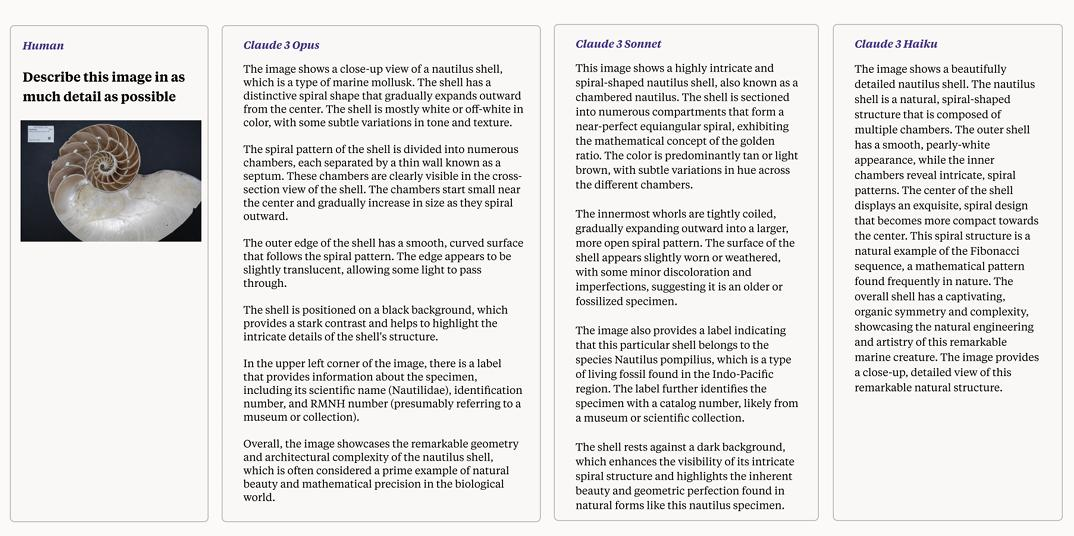
\includegraphics[width=0.85\textwidth]{claude3_vision_detection.png}
    \caption{Identificación de objetos visualmente usando modelos de Claude 3. Fuente: \cite{Anthropic2024}}
    \label{fig:claude3_detection}
\end{figure}

Claude 3 destaca en el reconocimiento óptico de caracteres (\textit{OCR}) en imágenes complejas, el procesamiento de documentos técnicos con \textit{layouts} sofisticados y la comprensión contextual de diagramas industriales, superando consistentemente a modelos anteriores en \textit{benchmarks} de comprensión documental \cite{Anthropic2024}.

El modelo exhibe capacidades avanzadas de razonamiento espacial que superan a sus predecesores en tareas que requieren comprensión de relaciones geométricas y propiedades físicas de objetos. Las evaluaciones técnicas independientes reportan un rendimiento superior en tareas de razonamiento espacial, con particular fortaleza en la interpretación de \textit{layouts} complejos y relaciones proporcionales entre elementos.

\begin{figure}[H]
    \centering
    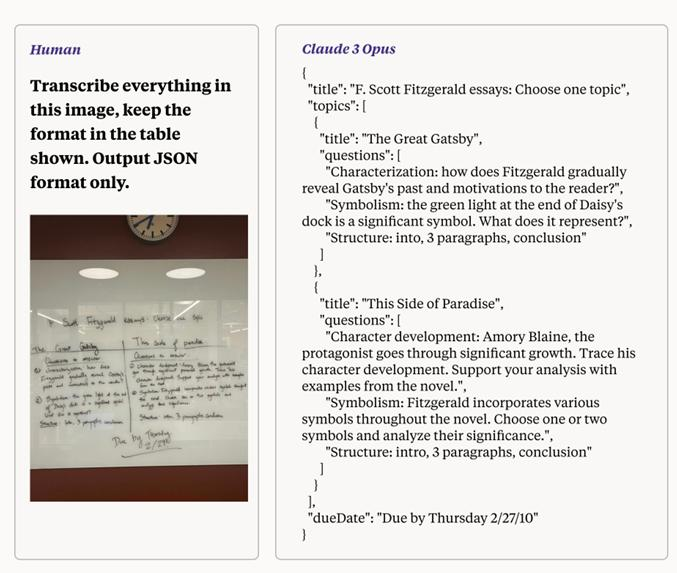
\includegraphics[width=0.85\textwidth]{claude3_json_output.png}
    \caption{Solicitud de reconocimiento de una imagen y reorganización en formato JSON.Fuente: \cite{Anthropic2024}}
    \label{fig:claude3_json}
\end{figure}

Para estimación dimensional, Claude 3 utiliza razonamiento contextual sofisticado que combina el reconocimiento de objetos conocidos con el análisis proporcional de elementos en la imagen. El sistema puede interpretar planos técnicos con dimensiones especificadas y extrapolar esta información para estimar las dimensiones de objetos fotografiados, logrando precisiones de $\pm$20--30\% en estimaciones sin referencias calibradas externas \cite{WebRef13251}.

La capacidad de procesamiento de documentos técnicos permite al modelo analizar especificaciones de productos, diagramas de embalaje y planos industriales, proporcionando estimaciones dimensionales basadas en la información contextual disponible en los documentos \cite{Anthropic2024}.

Claude 3 ofrece integración empresarial a través de la \textit{Anthropic API v1}, que proporciona \textit{endpoints RESTful} con autenticación basada en \textit{API keys} y límites de 4{,}000 tokens por minuto para todas las variantes del modelo. La \textit{API} soporta imágenes de hasta 20\,MB en formatos JPEG, PNG, GIF, WebP y PDF, facilitando la integración con sistemas existentes de gestión documental.

La arquitectura de la \textit{API} permite respuestas en múltiples formatos estructurados, incluyendo \textit{JSON}, texto estructurado y \textit{Markdown}, lo que facilita la integración con sistemas \textit{ERP}, plataformas de \textit{e-commerce} y aplicaciones de gestión logística. El sistema soporta procesamiento \textit{batch} para el análisis de grandes volúmenes de documentos y fotografías de inventario.

Las capacidades de \textit{streaming} permiten respuestas en tiempo real para aplicaciones interactivas, mientras que el modelo de \textit{pricing} por token de entrada y salida ofrece predictibilidad en los costos operacionales para implementaciones empresariales a gran escala.

Las implementaciones documentadas de Claude 3 en sectores logísticos y manufactureros incluyen aplicaciones específicas que aprovechan sus capacidades multimodales avanzadas:

\begin{itemize}
    \item \textbf{Análisis de especificaciones técnicas:} procesamiento automatizado de documentos de productos que incluyen planos técnicos con dimensiones especificadas, permitiendo extraer automáticamente información dimensional para sistemas de gestión de inventarios.
    \item \textbf{Interpretación de diagramas de embalaje:} análisis de documentos de \textit{packaging} que especifican configuraciones de empaque, permitiendo optimizar la utilización de espacio en contenedores y vehículos de transporte basándose en la interpretación visual de diagramas complejos.
    \item \textbf{Auditoría visual de inventarios:} procesamiento de fotografías de almacenes y centros de distribución para identificar discrepancias entre el inventario físico y los registros digitales, utilizando capacidades de reconocimiento de objetos y análisis espacial.
    \item \textbf{Análisis de documentos comerciales:} interpretación de facturas, órdenes de compra y documentos de envío que incluyen especificaciones de productos, automatizando la extracción de información dimensional crítica para procesos logísticos \cite{Anthropic2024}.
\end{itemize}

Las ventajas competitivas identificadas incluyen la ventana de contexto extendida (200K frente a 128K tokens de GPT-4), mejor comprensión de documentos complejos, razonamiento espacial más avanzado y menor tendencia a alucinaciones en datos técnicos críticos \cite{Anthropic2024}.

Las limitaciones operacionales incluyen una precisión dimensional comparable a GPT-4V ($\pm$20--30\%), dependencia de la calidad de imagen para un \textit{OCR} efectivo, costos por token potencialmente superiores a los de alternativas, y un ecosistema menos maduro de herramientas de terceros en comparación con OpenAI.


\subsubsection{Caso 3: Gemini 2.0 Flash}

Gemini 2.0 Flash, lanzado en diciembre de 2024, representa la segunda generación de modelos multimodales de Google con optimizaciones específicas para velocidad de procesamiento y análisis visual en tiempo real. El modelo incorpora una arquitectura \textit{transformer} multimodal de segunda generación optimizada para respuestas rápidas (denominación \textit{Flash}), logrando velocidades hasta 2$\times$ superiores a Gemini 1.0 en procesamiento multimodal \cite{Team20252, Team20251}.

El sistema soporta modalidades múltiples incluyendo texto, imagen, audio y video, con capacidad de procesamiento de imágenes de hasta 30\,MB en formatos \textit{JPEG}, \textit{PNG}, \textit{GIF}, \textit{WebP}, \textit{PDF}, \textit{SVG} y \textit{HEIC}. La ventana de contexto se expande masivamente a 2 millones de tokens, permitiendo el análisis simultáneo de múltiples documentos visuales complejos dentro de una sola sesión.

Las mejoras en análisis visual incluyen mejor razonamiento espacial, capacidades de análisis en tiempo real optimizadas y procesamiento simultáneo de hasta 20 objetos en una imagen individual, superando significativamente las limitaciones de 8--10 objetos de Gemini 1.0 \cite{Team20251}.


\begin{figure}[H]
    \centering
    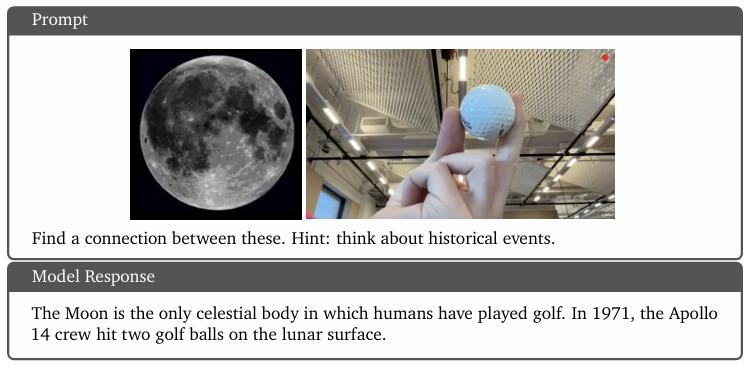
\includegraphics[width=0.9\textwidth]{gemini_multiimage_analysis.png}
    \caption{Se solicita a Gemini reconocer las imágenes y encontrar una relación entre ellas.}
    \label{fig:gemini_analysis}
\end{figure}

El sistema soporta modalidades múltiples incluyendo texto, imagen, audio y video, con capacidad de procesamiento de imágenes de hasta 30MB en formatos JPEG, PNG, GIF, WebP, PDF, SVG y HEIC. La ventana de contexto se expande masivamente a 2 millones de tokens.

Gemini 2.0 Flash integra Google Lens como módulo nativo, eliminando la arquitectura de integración externa de generaciones anteriores. El sistema demuestra precisión mejorada en estimaciones dimensionales, alcanzando márgenes de $\pm$8--15\% con objetos de referencia en productos estándar, $\pm$5--12\% en condiciones de laboratorio controlado, y $\pm$12--25\% en uso típico de usuarios reales \cite{Team20252}.

Implementaciones específicas en logística incluyen:
\begin{itemize}
    \item Análisis de inventario en tiempo real para Google Shopping
    \item Medición automatizada de productos para Google Merchant Center
    \item Optimización de embalaje en centros de distribución
    \item Análisis de fotografías de productos para Google Lens Shopping
\end{itemize}

\subsubsection{Caso 4: Vision Transformer (ViT) para reconocimiento y dimensionado de productos}

Vision Transformer (ViT), introducido por Dosovitskiy et al. en Google Research (2020) y publicado en ICLR 2021, revolucionó el campo de \textit{computer vision} al demostrar que arquitecturas transformer puras pueden superar las redes neuronales convolucionales tradicionales en tareas de reconocimiento de imágenes. El modelo alcanza 94.2\% de precisión en \textit{ImageNet classification} cuando se \textit{pre-entrena} en \textit{datasets} suficientemente grandes \cite{Dosovitskiy2020}.

La arquitectura divide imágenes en \textit{patches} de 16$\times$16 píxeles que se procesan como secuencias, similar al procesamiento de tokens en modelos de lenguaje. Esta metodología permite \textit{transfer learning} eficiente para nuevas categorías de productos.

Las implementaciones académicas posteriores han demostrado aplicabilidad directa en \textit{retail analytics}. DINOv2 (Meta AI Research, 2023) introduce \textit{self-supervised learning} que elimina la dependencia de datasets etiquetados masivos, logrando representaciones visuales robustas especialmente efectivas para reconocimiento de productos \cite{Oquab2024}.

Para estimación dimensional, las investigaciones académicas reportan precisiones de $\pm$12--18\% en objetos con referencias visuales, utilizando visual \textit{reasoning} sobre \textit{features transformer} que capturan relaciones espaciales complejas.

% ------------------------------------------------------------------
\subsection{Aplicaciones de LLMs multimodal en logística y comercio electrónico}
% ------------------------------------------------------------------

Florence (Microsoft Research, 2021) establece un framework multimodal que combina \textit{vision transformers} con capacidades de lenguaje natural, demostrando aplicabilidad directa para tareas que requieren comprensión semántica de productos y estimación de propiedades físicas.

Las evaluaciones académicas independientes confirman escalabilidad para procesamiento de millones de productos, con implementaciones que mantienen eficiencia computacional mediante técnicas de \textit{patch embedding} optimizadas.

% ------------------------------------------------------------------
\section{Características de soluciones semejantes o similares}
% ------------------------------------------------------------------

\subsection{Arquitecturas de procesamiento predominantes}

Las soluciones analizadas convergen en arquitecturas de procesamiento que combinan múltiples enfoques tecnológicos. Los sistemas comerciales líderes utilizan \textit{transformers} multimodal que integran vision encoders especializados (CLIP, ALIGN, ViT) con \textit{large language models} para interpretación semántica avanzada.

Las implementaciones actuales emplean \textit{attention mechanisms cross-modal} que permiten correlación directa entre características visuales y comprensión textual, facilitando estimación dimensional mediante razonamiento contextual \cite{Dosovitskiy2020}.

\subsection{Capacidades de interpretación dimensional}

Las capacidades de interpretación dimensional se fundamentan en:

\begin{enumerate}
    \item \textbf{Reconocimiento automático de referencias de escala}: Los modelos identifican objetos conocidos (monedas, tarjetas, manos humanas) para establecer proporciones relativas.
    \item \textbf{Análisis de perspectiva y profundidad visual}: Utiliza \textit{depth estimation} implícito derivado de características de textura y sombras.
    \item \textbf{Razonamiento contextual sofisticado}: Combina reconocimiento de objetos conocidos con análisis proporcional de elementos en la imagen \cite{Oquab2024}.
\end{enumerate}

\subsection{Precisión y confiabilidad según implementación}

La precisión varía significativamente según la implementación y condiciones operacionales:

\begin{table}[H]
\centering
\caption{Comparativa de precisión por tipo de sistema.}
\label{tab:precision_sistemas}
\begin{tabular}{@{}lcc@{}}
\toprule
\textbf{Tipo de Sistema} & \textbf{Condiciones Óptimas} & \textbf{Condiciones Reales} \\
\midrule
LLMs multimodal & $\pm$10--25\% & $\pm$15--30\% \\
Vision Transformers & $\pm$12--18\% & $\pm$15--25\% \\
Sistemas con hardware & $\pm$2--5mm & $\pm$5--10mm \\
\bottomrule
\end{tabular}
\end{table}

La degradación de precisión con iluminación deficiente, ángulos subóptimos y \textit{backgrounds} complejos representa un desafío común.

% ------------------------------------------------------------------
\section{Compendio de tecnologías, herramientas, métodos, modelos utilizados con éxito}
% ------------------------------------------------------------------

\subsection{Modelos de lenguaje multimodal predominantes}

\textbf{Modelos de gran escala comerciales:}
\begin{itemize}
    \item GPT-4 Vision (OpenAI) - 1.76 trillones de parámetros
    \item Claude Sonnet 4 (Anthropic) - Optimizado para razonamiento visual
    \item Gemini 2.0 Flash (Google) - Optimizaciones de velocidad
    \item LLaVA - Alternativas \textit{open-source}
\end{itemize}

\textbf{Arquitecturas especializadas predominantes:}
\begin{itemize}
    \item CLIP (\textit{Contrastive Language-Image Pre-training})
    \item BLIP-2 (\textit{Bootstrapped vision-language pre-training})
    \item InstructBLIP - Seguimiento de instrucciones específicas
    \item MiniGPT-4 - Eficiencia en recursos limitados
\end{itemize}

\subsection{Frameworks de visión por computadora académicos}

Vision Transformers (ViT) representan el estado del arte en análisis visual académico:

\begin{itemize}
    \item ViT-Base: 86 millones de parámetros
    \item ViT-Large: 307 millones de parámetros
    \item ViT-Huge: 632 millones de parámetros
\end{itemize}

Modelos híbridos incluyen DeiT (\textit{Data-efficient image Transformers}), Swin Transformer optimizado para imágenes de alta resolución, y EfficientViT diseñado para implementaciones móviles.

\subsection{Tecnologías de infraestructura en la nube}

\textbf{Plataformas de IA como servicio:}
\begin{itemize}
    \item OpenAI API con GPT-4 Vision endpoints
    \item Anthropic Claude API para análisis multimodal
    \item Google Vertex AI con modelos Gemini integrados
    \item Azure Cognitive Services
    \item AWS Bedrock
\end{itemize}

\textbf{Servicios de computación distribuida:}
\begin{itemize}
    \item AWS Lambda - Procesamiento \textit{serverless}
    \item Google Cloud Run - Containerización
    \item Azure Container Instances - Escalabilidad elástica
    \item Kubernetes - Orquestación de microservicios
\end{itemize}

\subsection{Herramientas de desarrollo e integración}

\textbf{Bibliotecas de integración:}
\begin{itemize}
    \item LangChain - Framework para aplicaciones LLM
    \item LlamaIndex - \textit{Retrieval-Augmented Generation}
    \item Haystack - Pipelines \textit{end-to-end}
    \item Transformers (HuggingFace) - Acceso a modelos pre-entrenados
\end{itemize}

\textbf{SDKs para desarrollo móvil:}
\begin{itemize}
    \item React Native con plugins para APIs de IA
    \item Flutter con packages para computer vision
    \item Swift/Kotlin con SDKs nativos
    \item Progressive Web Apps para acceso universal
\end{itemize}

\subsection{Metodologías de prompt engineering y optimización}

\textbf{Técnicas avanzadas de diseño de prompts:}
\begin{itemize}
    \item \textit{Few-shot learning} para medición dimensional
    \item \textit{Chain-of-thought prompting} para razonamiento paso a paso
    \item \textit{Structured output formatting} para consistencia
    \item \textit{Multi-turn conversation} para refinación iterativa
\end{itemize}

\textbf{Estrategias de optimización:}
\begin{itemize}
    \item \textit{Fine-tuning} con datos del dominio logístico
    \item \textit{Retrieval-Augmented Generation} (RAG)
    \item \textit{In-context learning} con ejemplos calibrados
    \item LoRA y Adapters para personalización eficiente
\end{itemize}

% ------------------------------------------------------------------
\section{Conjunto de características y especificaciones para la solución óptima}
% ------------------------------------------------------------------

\subsection{Arquitectura tecnológica óptima}

Basándose en el análisis de soluciones existentes, la arquitectura óptima debe combinar:

\begin{itemize}
    \item Modelos de lenguaje multimodal de última generación
    \item Infraestructura \textit{cloud} escalable
    \item Procesamiento distribuido eficiente
    \item Interfaces móviles intuitivas
\end{itemize}

\subsection{Precisión y confiabilidad requeridas}

Para aplicaciones logísticas comerciales, el sistema debe alcanzar:

\begin{itemize}
    \item Precisión de $\pm$15--20\% en condiciones reales de uso
    \item Mejora a $\pm$10--15\% con referencias de escala adecuadas
    \item Tiempos de respuesta inferiores a 5 segundos
    \item Disponibilidad superior al 99.5\%
\end{itemize}

Esta precisión es suficiente para categorización de tarifas de envío, optimización básica de carga vehicular, y estimaciones de costos logísticos sin requerir inversión en hardware especializado.

\subsection{Limitaciones y alcances reconocidos}

El sistema está diseñado para:

\begin{itemize}
    \item Estimaciones dimensionales aproximadas para categorización logística
    \item Paquetes regulares de e-commerce (5cm a 2 metros)
    \item Condiciones de iluminación mínima adecuada
    \item Mercado peruano inicialmente, con escalabilidad regional
\end{itemize}

Limitaciones reconocidas:

\begin{itemize}
    \item No apto para aplicaciones que requieran precisión milimétrica
    \item Degradación con objetos transparentes o altamente reflectivos
    \item Requiere iluminación mínima adecuada
    \item Formas extremadamente irregulares presentan mayor error
\end{itemize}

% cSpell:language es,en
% ==================================================================
% CAPÍTULO 3: DISEÑO DE LA SOLUCIÓN AL DESAFÍO DE INGENIERÍA
% ==================================================================

\chapter{Diseño de la solución al desafío de ingeniería}

% ------------------------------------------------------------------
% INTRODUCCIÓN AL CAPÍTULO
% ------------------------------------------------------------------

El capítulo describe el diseño de la solución técnica al problema de la estimación manual e inexacta de dimensiones de paquetes en pymes de \textit{delivery} en Lima. Basado en la metodología Design Thinking, el proceso asegura que cada decisión técnica responda a las necesidades reales de los usuarios y al contexto local.

Se siguen cuatro fases del método aplicadas al diseño: Empatizar, Definir, Idear y Prototipar, dejando la fase de Evaluación para el siguiente capítulo donde se analizará la viabilidad técnica, económica y social de la solución diseñada.

Cada etapa genera entregables que reflejan las competencias del Ingeniero de Telecomunicaciones de la PUCP, vinculando el diseño con el perfil profesional. El capítulo cierra con una reflexión crítica sobre fortalezas, limitaciones y mejoras futuras, sentando la base para la implementación del sistema.

% ------------------------------------------------------------------
\section{Introducción metodológica – Enfoque Design Thinking}
% ------------------------------------------------------------------

\subsection{Justificación del enfoque centrado en el usuario}

La aplicación de Design Thinking en este proyecto de ingeniería de telecomunicaciones permite equilibrar la complejidad técnica con las necesidades reales de las pymes de \textit{delivery} en Lima. Este enfoque integra el rigor de la ingeniería —infraestructura cloud, latencia, disponibilidad, escalabilidad y optimización en dispositivos móviles— con la comprensión de las condiciones operativas reales, evitando soluciones avanzadas pero inviables o desconectadas del contexto. 

Su carácter iterativo facilita ajustes basados en retroalimentación, garantizando una solución técnicamente robusta, económicamente viable y adoptable, alineada con las competencias profesionales del ingeniero de telecomunicaciones y los Objetivos de Desarrollo Sostenible.

\subsection{Fases de Design Thinking aplicadas en este capítulo}

Este capítulo desarrolla cuatro de las cinco fases del Design Thinking, enfocándose en el diseño de la solución:

\begin{itemize}
    \item \textbf{Empatizar}: Se busca comprender las necesidades reales de los usuarios, identificando los problemas operativos que enfrentan las empresas de \textit{delivery} al estimar manualmente las dimensiones de paquetes.
    
    \item \textbf{Definir}: Se establecen los requerimientos funcionales y no funcionales que debe cumplir el sistema de gestión logística a partir de los hallazgos obtenidos.
    
    \item \textbf{Idear}: Se evalúan múltiples alternativas tecnológicas mediante criterios de escalabilidad, costo y viabilidad para seleccionar la solución óptima.
    
    \item \textbf{Prototipar}: Se materializa el diseño técnico detallado, incluyendo la arquitectura de sistema, modelo de datos, módulo de IA y especificaciones de red.
\end{itemize}

% ------------------------------------------------------------------
\section{Fase 1: Empatizar – Análisis del contexto y usuarios}
% ------------------------------------------------------------------

\subsection{Contexto del problema y metodología de investigación}

\subsubsection{Contexto geográfico e institucional}

El proyecto se desarrolla en el contexto de las pequeñas y medianas empresas de \textit{delivery} que operan en Lima, Perú, una ciudad de alta densidad urbana. El mercado logístico local se caracteriza por la predominancia de procesos manuales, la alta informalidad, el uso intensivo de motorizados en motocicletas para entregas de último kilómetro y una creciente demanda de servicios de \textit{delivery} impulsada por el comercio electrónico.

Estas empresas operan sin sistemas tecnológicos integrados, dependiendo de la comunicación por WhatsApp, los registros en hojas de cálculo y la coordinación telefónica, lo que genera ineficiencias, falta de trazabilidad y dificultades para escalar sus operaciones.

\subsubsection{Técnicas de investigación aplicadas}

Para comprender el contexto y las necesidades de los usuarios, se aplicaron dos técnicas principales:

\begin{enumerate}
    \item \textbf{Análisis del flujo logístico}: Se estudió el proceso desde el registro de pedidos hasta la entrega final en pequeñas empresas de \textit{delivery}, identificando ineficiencias y oportunidades de automatización.
    
    \item \textbf{Análisis comparativo de soluciones}: Se evaluaron las herramientas tecnológicas existentes, tanto informales como comerciales, analizando sus funciones, limitaciones y costos. Este análisis evidenció vacíos en las herramientas actuales y oportunidades para integrar tecnologías emergentes como la inteligencia artificial multimodal.
\end{enumerate}

\subsubsection{Actores clave del sistema}

El análisis identificó cinco actores clave en el sistema:

\begin{itemize}
    \item \textbf{Clientes emisores}: Solicitan envíos y requieren transparencia en costos y trazabilidad de sus pedidos.
    
    \item \textbf{Administradores}: Gestionan la operación logística y necesitan herramientas para supervisión centralizada, asignación eficiente de recursos y toma de decisiones basada en datos.
    
    \item \textbf{Motorizados}: Ejecutan las entregas en campo y demandan información clara sobre asignaciones, rutas optimizadas y herramientas para registrar evidencias.
    
    \item \textbf{Destinatarios}: Reciben los paquetes y esperan puntualidad e información sobre el estado de su entrega.
\end{itemize}

La tabla del Anexo A detalla el rol específico de cada actor, sus necesidades principales y los problemas operativos actuales que enfrentan, información fundamental para la definición de requerimientos del sistema. Esta caracterización exhaustiva de actores permite asegurar que el diseño técnico considere las perspectivas de todos los usuarios que interactuarán con el sistema, desde la interfaz móvil optimizada para operación en campo por motorizados hasta el dashboard web con análisis en tiempo real para administradores.

\subsection{Síntesis de hallazgos}

La fase de empatía reveló hallazgos críticos organizados en tres categorías que fundamentan el diseño técnico posterior: necesidades identificadas, restricciones del contexto y oportunidades de mejora mediante tecnología. Estos hallazgos, desarrollados en el Anexo B, representan la transformación de observaciones cualitativas en insumos estructurados que guiarán las decisiones de arquitectura, selección de tecnologías y priorización de funcionalidades en las fases subsecuentes del proceso de diseño.

Estos hallazgos revelan que el desafío técnico trasciende la simple automatización de mediciones, representando una oportunidad para transformar integralmente la gestión logística de pequeñas empresas mediante tecnologías de telecomunicaciones modernas que hasta ahora estaban reservadas para empresas con grandes presupuestos tecnológicos.

% ------------------------------------------------------------------
\section{Fase 2: Definir – Reformulación del problema técnico}
% ------------------------------------------------------------------

\subsection{Declaración del problema de ingeniería}

Con base en los hallazgos de la fase de empatía, se formula el siguiente problema técnico:

Las pequeñas y medianas empresas de \textit{delivery} en Lima enfrentan ineficiencias operativas derivadas de la estimación manual e inexacta de dimensiones de paquetes, la falta de trazabilidad en tiempo real de las entregas, y la gestión desarticulada mediante herramientas informales (WhatsApp, hojas de cálculo). Esta problemática genera costos ocultos por viajes innecesarios, insatisfacción de clientes por reprogramaciones, y limitaciones para escalar operaciones.

Desde la perspectiva de ingeniería de telecomunicaciones, se requiere diseñar una arquitectura distribuida que integre procesamiento de imágenes con inteligencia artificial en la nube y aplicaciones móviles, todo bajo un modelo económicamente viable para empresas emergentes y cumpliendo con normativas de protección de datos personales.

\subsection{Requerimientos funcionales del sistema}



\begin{longtable}{@{}p{3.5cm}p{1.5cm}p{10cm}@{}}
\caption{Requisitos funcionales del sistema} \\
\toprule
\textbf{Categoría} & \textbf{Código} & \textbf{Descripción} \\ 
\midrule
\endfirsthead

\multicolumn{3}{c}%
{\tablename\ \thetable{} -- continuación de la página anterior} \\
\toprule
\textbf{Categoría} & \textbf{Código} & \textbf{Descripción} \\ 
\midrule
\endhead

\midrule \multicolumn{3}{r}{{Continúa en la siguiente página}} \\ 
\bottomrule
\endfoot

\bottomrule
\endlastfoot

% ---------- CONTENIDO DE LA TABLA ----------

\multirow{4}{=}{Gestión de usuarios y roles} 
& RF1.1 & El sistema debe permitir el registro y autenticación de usuarios. \\
& RF1.2 & El sistema debe permitir que el Administrador gestione pedidos, usuarios y visualice motorizados en tiempo real. \\
& RF1.3 & El sistema debe permitir que el Cliente cree pedidos, registre datos y suba fotos. \\
& RF1.4 & El sistema debe permitir que el Motorizado reciba y actualice el estado de pedidos asignados. \\ \midrule

\multirow{5}{=}{Gestión de pedidos} 
& RF2.1 & El cliente debe poder crear pedidos en el sistema, incluyendo dirección de recojo, dirección de entrega, cliente, foto, celular y distrito. \\
& RF2.2 & Al crear un pedido, el cliente debe subir fotos del paquete. \\
& RF2.3 & El sistema debe procesar las fotos usando IA multimodal para detectar objetos de referencia y calcular dimensiones. \\
& RF2.4 & El sistema debe guardar las dimensiones junto con la información del pedido y permitir su edición manual. \\
& RF2.5 & El administrador debe poder asignar pedidos a un motorizado. \\ \midrule

\multirow{5}{=}{Gestión de motorizados} 
& RF3.1 & El motorizado debe visualizar en la aplicación móvil los pedidos asignados. \\
& RF3.2 & El motorizado debe poder capturar foto en el recojo del pedido (evidencia). \\
& RF3.3 & El motorizado debe poder capturar foto en la entrega (evidencia). \\
& RF3.4 & El sistema debe cambiar automáticamente el estado del pedido al capturar fotos de evidencia. \\
& RF3.5 & El motorizado puede visualizar los pedidos en un mapa. \\ \midrule

\multirow{3}{=}{Dashboard Web (administrador)} 
& RF4.1 & El administrador debe visualizar en un dashboard la lista de pedidos, estados, dimensiones, fotos y motorizado asignado. \\
& RF4.2 & El dashboard debe permitir filtrar pedidos por estado, cliente o motorizado. \\
& RF4.3 & El administrador debe poder visualizar la ubicación en tiempo real de los motorizados en un mapa dentro del dashboard web. \\ \midrule

\multirow{2}{=}{Notificaciones y sincronización} 
& RF5.1 & El motorizado debe recibir notificaciones push automáticas cuando se le asigne un nuevo pedido. \\
& RF5.2 & El cliente debe recibir notificaciones push sobre cambios de estado del pedido. \\ \midrule

\multirow{2}{=}{Seguridad y consistencia} 
& RF6.1 & El sistema debe asegurar el acceso por roles (cada usuario solo ve lo que le corresponde). \\
& RF6.2 & El sistema debe cifrar las comunicaciones mediante TLS y proteger el acceso a datos mediante reglas de seguridad de Firebase. \\

\end{longtable}

\subsection{Requisitos no funcionales}

\begin{longtable}{@{}p{3.5cm}p{1.5cm}p{10cm}@{}}
\caption{Requisitos no funcionales del sistema} \\
\toprule
\textbf{Categoría} & \textbf{Código} & \textbf{Descripción} \\ 
\midrule
\endfirsthead

\multicolumn{3}{c}%
{\tablename\ \thetable{} -- continuación de la página anterior} \\
\toprule
\textbf{Categoría} & \textbf{Código} & \textbf{Descripción} \\ 
\midrule
\endhead

\midrule \multicolumn{3}{r}{{Continúa en la siguiente página}} \\ 
\bottomrule
\endfoot

\bottomrule
\endlastfoot

% ---------- CONTENIDO ----------

\multirow{2}{=}{Rendimiento}
& RNF1.1 & El sistema debe procesar la estimación de dimensiones de un paquete mediante IA en menos de 10 segundos después de subir la foto. \\
& RNF1.2 & El dashboard web debe cargar la información principal en menos de 5 segundos. \\ \midrule

\multirow{2}{=}{Disponibilidad}
& RNF2.1 & El sistema debe mantener una disponibilidad mínima del 99.5\% aprovechando la infraestructura cloud de Firebase. \\
& RNF2.2 & Debe existir backup automático de datos en Firebase para evitar pérdida de información. \\ \midrule

\multirow{3}{=}{Seguridad}
& RNF3.1 & Toda comunicación entre cliente y servidor debe usar cifrado SSL/TLS (implementado por defecto en Firebase). \\
& RNF3.2 & Las contraseñas deben almacenarse de forma segura mediante Firebase Auth. \\
& RNF3.3 & El acceso a datos debe estar protegido mediante reglas de seguridad basadas en roles. \\ \midrule

\multirow{2}{=}{Compatibilidad}
& RNF4.1 & La aplicación móvil debe ser compatible con dispositivos Android 12.0 (API level 31) o superior, considerando el uso de terminales de gama media a baja. \\
& RNF4.2 & El dashboard web debe funcionar correctamente en navegadores modernos (Chrome, Firefox, Edge). \\ \midrule

\multirow{2}{=}{Usabilidad}
& RNF5.1 & La interfaz debe ser intuitiva y permitir completar las tareas principales sin necesidad de capacitación extensa. \\
& RNF5.2 & Los mensajes de error deben ser claros y comprensibles. \\ \midrule

\multirow{2}{=}{Fiabilidad del Modelo de IA}
& RNF6.1 & El modelo de IA debe tener un error promedio menor al 20\% en la estimación de dimensiones cuando se proporciona un objeto de referencia reconocible. \\
& RNF6.2 & El sistema debe permitir corrección manual de las dimensiones estimadas. \\ \midrule

\multirow{5}{=}{Cumplimiento Legal}
& RNF7.1 & El sistema debe cumplir con la Ley N.º 29733 - Ley de Protección de Datos Personales del Perú. \\
& RNF7.2 & Debe implementarse un consentimiento informado al registrar usuarios, indicando qué datos personales se recopilan, para qué se utilizan, quién tendrá acceso y los derechos ARCO. \\
& RNF7.3 & Las fotografías de paquetes y evidencias deben almacenarse de forma segura y solo ser accesibles por usuarios autorizados. \\
& RNF7.4 & Los datos de ubicación de motorizados solo deben ser visibles durante entregas activas. \\
& RNF7.5 & Debe existir una Política de Privacidad clara y accesible en la aplicación. \\ \midrule

\multirow{2}{=}{Mantenibilidad}
& RNF8.1 & El código debe estar documentado para facilitar su comprensión y futuras modificaciones. \\
& RNF8.2 & El sistema debe generar logs básicos de errores críticos. \\ \midrule

\multirow{3}{=}{Eficiencia de recursos}
& RNF9.1 & Las imágenes capturadas deben comprimirse automáticamente a un tamaño máximo de 500KB para minimizar el uso de datos móviles. \\
& RNF9.2 & El procesamiento intensivo (análisis de IA) debe ejecutarse en el backend (Cloud Functions) para no sobrecargar dispositivos de recursos limitados. \\
& RNF9.3 & La aplicación debe utilizar thumbnails (máximo 30KB) en listas y cargar imágenes completas solo cuando el usuario lo solicite explícitamente. \\

\end{longtable}

\subsection{Matriz de trazabilidad: necesidades vs. requerimientos}

La tabla en el anexo C establece la trazabilidad entre las necesidades identificadas en la fase de empatía y los requerimientos funcionales y no funcionales definidos, asegurando que cada necesidad del usuario tenga una respuesta técnica específica en el diseño.

\subsection{Restricciones de diseño}

Las restricciones identificadas en la fase de empatía condicionan las decisiones técnicas del diseño de la solución y establecen los límites operativos, normativos y éticos dentro de los cuales debe funcionar el sistema.

\subsubsection{Restricciones económicas}

Las microempresas de \textit{delivery} requieren tecnologías de bajo costo que respalden su operación sin comprometer su sostenibilidad financiera. Dado su limitado presupuesto y la necesidad de costos operativos escalables, no pueden asumir gastos fijos elevados por infraestructura o licencias. Por ello, esta tesis emplea las capas gratuitas de servicios cloud (Firebase Free Tier) para desarrollar, prototipar y validar la solución sin incurrir en costos significativos durante la fase académica.

\subsubsection{Restricciones técnicas}

Los motorizados operan con conectividad móvil variable (3G/4G intermitente) en los distintos distritos de Lima, dependiendo del operador contratado y la cobertura disponible en cada zona. Esta condición externa no está bajo control del presente desarrollo, ya que responde a la infraestructura de telecomunicaciones existente. Dado el uso predominante de dispositivos Android de gama media a baja, el sistema debe contemplar capacidades de procesamiento en el borde (edge), permitiendo la compresión y reducción de imágenes antes de su envío a la nube, con el fin de optimizar el uso de datos y garantizar la viabilidad operativa.

\subsubsection{Restricciones operativas}

Los motorizados requieren flujos de interacción simples y ágiles durante las operaciones de recojo y entrega, realizadas en exteriores con condiciones variables. La aplicación debe funcionar eficientemente en dispositivos móviles estándar, sin depender de capacitación extensa, considerando la alta rotación de personal en el sector logístico. Esta restricción se aborda desde el diseño funcional del sistema, sin profundizar en aspectos de interfaz gráfica.

\subsubsection{Restricciones normativas}

El sistema gestiona información sensible como teléfonos, direcciones, razón social, imágenes y evidencias de entrega, por lo que debe cumplir estrictamente con la Ley N.º 29733 de Protección de Datos Personales. Esto incluye consentimiento informado al registro, definición clara de uso y acceso a datos, y respeto a los derechos ARCO (Acceso, Rectificación, Cancelación, Oposición).

Las imágenes procesadas por IA se almacenan en Firebase Storage con reglas de acceso por rol, y los datos de ubicación de motorizados solo se visualizan durante entregas activas, sin persistencia innecesaria.

\subsubsection{Restricciones éticas}

Las imágenes procesadas por el módulo de inteligencia artificial se utilizarán exclusivamente para estimar dimensiones de paquetes, garantizando un uso ético y limitado de esta información sensible. No se emplearán para entrenar modelos externos, compartir con terceros ni otros fines distintos a los declarados. El sistema debe informar claramente a los usuarios sobre el análisis automatizado de sus fotografías y aplicar políticas de minimización de datos para proteger la privacidad de personas que pudieran aparecer incidentalmente.

\subsubsection{Restricciones de alcance y tiempo}

El proyecto se desarrollará en un plazo estimado de cinco meses, centrado en construir un prototipo funcional que permita validar la propuesta técnica. Se priorizan funcionalidades esenciales como gestión de usuarios y roles, seguimiento de pedidos, medición automática de dimensiones con IA, asignación a motorizados, registro de evidencias y trazabilidad básica en tiempo real.

No se incluyen optimizaciones avanzadas ni características empresariales como reportes analíticos, integraciones con ERP, facturación o analítica predictiva, las cuales se consideran fuera del alcance comprometido y posibles extensiones futuras. El enfoque se limita a una experiencia operativa suficiente para evaluar la viabilidad técnica del sistema.

\subsection{Arquitectura conceptual del sistema}

Basándose en los requerimientos funcionales y no funcionales definidos, el sistema requiere una arquitectura distribuida compuesta por:

\begin{itemize}
    \item \textbf{Capa de presentación}: App móvile y App web
    \item \textbf{Capa de lógica de negocio}: Procesamiento serverless, funciones serverless
    \item \textbf{Capa de datos}: Base de datos, almacenamiento de archivos, autenticación
    \item \textbf{Capa de servicios}: Geolocalización, notificaciones, procesamiento IA
\end{itemize}

\begin{figure}[H]
    \centering
    \begin{tikzpicture}[
        node distance=0.8cm and 1.2cm,
        box/.style={rectangle, draw=gray!70, rounded corners, minimum width=3cm, minimum height=1cm, align=center, fill=blue!5},
        layerbox/.style={rectangle, draw=gray!60, rounded corners, minimum width=13cm, minimum height=2cm, align=center, fill=gray!10},
        label/.style={font=\small\bfseries, anchor=south west, text=black}
    ]
    
    % CAPA DE PRESENTACIÓN
    \node[layerbox] (capa1) {};
    \node[label] at (capa1.north west) [yshift=0.3cm] (label1) {CAPA DE PRESENTACIÓN};
    \node[box] (appmov) at ([xshift=-2cm]capa1.center) {App móvil};
    \node[box] (appweb) at ([xshift=2cm]capa1.center) {App web};
    
    % LÓGICA DE NEGOCIO
    \node[layerbox, below=1.3cm of capa1, fill=blue!5!gray!10] (capa2) {};
    \node[label] at (capa2.north west) [yshift=0.3cm] (label2) {LÓGICA DE NEGOCIO};
    \node[box, fill=blue!10] (proc) at ([xshift=-2cm]capa2.center) {Procesamiento\\Serverless};
    \node[box, fill=blue!10] (func) at ([xshift=2cm]capa2.center) {Función Serverless};
    
    % CAPA DE DATOS
    \node[layerbox, below=1.3cm of capa2, fill=green!5!gray!10] (capa3) {};
    \node[label] at (capa3.north west) [yshift=0.3cm] (label3) {CAPA DE DATOS};
    \node[box, fill=green!10] (alm) at ([xshift=-4cm]capa3.center) {Almacenamiento de\\archivos};
    \node[box, fill=green!10] (aut) at (capa3.center) {Autenticación};
    \node[box, fill=green!10] (bd) at ([xshift=4cm]capa3.center) {Base de datos};
    
    % CAPA DE SERVICIOS
    \node[layerbox, below=1.3cm of capa3, fill=orange!5!gray!10] (capa4) {};
    \node[label] at (capa4.north west) [yshift=0.3cm] (label4) {CAPA DE SERVICIOS};
    \node[box, fill=orange!10] (not) at ([xshift=-4cm]capa4.center) {Notificaciones};
    \node[box, fill=orange!10] (geo) at (capa4.center) {Geolocalización};
    \node[box, fill=orange!10] (ia) at ([xshift=4cm]capa4.center) {Procesamiento IA};
    
    % Flechas de conexión
    \draw[->, thick, gray!70] (capa1) -- (capa2);
    \draw[->, thick, gray!70] (capa2) -- (capa3);
    \draw[->, thick, gray!70] (capa3) -- (capa4);
    \end{tikzpicture}
    \caption{Arquitectura de capas del sistema}
    \label{fig:arquitectura-capas}
    {\small \textit{Fuente:} Elaboración propia}
\end{figure}



Esta arquitectura conceptual será materializada en la Fase 3 mediante la evaluación de alternativas tecnológicas específicas.

% ------------------------------------------------------------------
\section{Fase 3: Idear – Generación y selección de alternativas}
% ------------------------------------------------------------------

\subsection{Introducción a la generación de alternativas}

Con los requerimientos definidos, la fase de ideación evalúa alternativas tecnológicas que respondan a las necesidades identificadas. Se comparan sistemáticamente opciones de arquitectura, telecomunicaciones, plataformas cloud y enfoques de implementación mediante criterios técnicos, económicos y operativos. Este análisis multicriterio permite justificar la solución seleccionada con rigor ingenieril, evitando decisiones basadas en preferencias subjetivas o familiaridad tecnológica.

\subsection{Criterios de evaluación}

Para la evaluación de alternativas se establecen seis criterios principales que reflejan los requerimientos y restricciones identificados en la fase anterior:

\begin{table}[H]
\centering
\caption{Criterios de evaluación de alternativas tecnológicas.}
\label{tab:criterios_evaluacion}
\begin{tabular}{@{}p{2.5cm}p{5cm}p{1.5cm}p{4cm}@{}}
\toprule
\textbf{Criterio} & \textbf{Descripción} & \textbf{Peso} & \textbf{Justificación} \\
\midrule
Escalabilidad & Capacidad del sistema para crecer automáticamente con la demanda sin requerir reconfiguración manual significativa & 20\% & Fundamental para pequeñas empresas que planean crecer progresivamente sin inversiones disruptivas \\
\midrule
Costo & Inversión inicial, costos operativos mensuales y modelo de pago (fijo vs. variable) & 25\% & Criterio crítico dado el presupuesto limitado de las empresas objetivo y el uso de capas gratuitas para el desarrollo de tesis \\
\midrule
Facilidad de integración & Complejidad de integrar los diferentes componentes del sistema y tiempo de desarrollo requerido & 15\% & Importante considerando el plazo de 5 meses para el desarrollo de la tesis \\
\midrule
Mantenimiento & Esfuerzo requerido para mantener la infraestructura, actualizar componentes y gestionar la seguridad & 15\% & Relevante para empresas pequeñas con recursos técnicos limitados \\
\midrule
Rendimiento & Latencia, throughput y tiempo de respuesta del sistema en condiciones reales de uso & 15\% & Necesario para garantizar experiencia de usuario aceptable y sincronización en tiempo real \\
\midrule
Ecosistema y soporte & Disponibilidad de documentación, comunidad de desarrolladores, SDKs y herramientas de desarrollo & 10\% & Facilita la resolución de problemas y reduce riesgos durante la implementación \\
\bottomrule
\end{tabular}
\end{table}

\subsection{Alternativas consideradas}

Se identifican tres alternativas principales de arquitectura que cumplen con los requerimientos funcionales establecidos.

\subsubsection{Alternativa 1: Ecosistema Firebase/Google Cloud}

\textbf{Descripción técnica}: Arquitectura completamente basada en servicios de Google Cloud Platform, utilizando Firebase como Backend-as-a-Service (BaaS). Los componentes principales incluyen: Firebase Firestore (base de datos NoSQL en tiempo real), Firebase Authentication (gestión de usuarios y roles), Firebase Storage (almacenamiento de imágenes), Firebase Cloud Functions (lógica serverless), Firebase Cloud Messaging (notificaciones push), Firebase Hosting (dashboard web), Google Maps API (geolocalización), y integración con modelos de IA multimodal (Gemini, Claude, GPT-4 Vision) mediante Cloud Functions.

\textbf{Arquitectura de telecomunicaciones}:
\begin{itemize}
    \item Sincronización en tiempo real mediante WebSockets gestionados por Firestore
    \item Protocolo HTTPS/TLS para todas las comunicaciones
    \item CDN global de Google para distribución de contenido estático
    \item Latencia típica de 50-200ms según ubicación geográfica
    \item Escalamiento automático horizontal sin configuración
\end{itemize}

\textbf{Ventajas}:
\begin{itemize}
    \item Integración nativa entre todos los componentes del ecosistema
    \item Capa gratuita generosa para desarrollo y validación de tesis
    \item Sincronización en tiempo real nativa (offline-first)
    \item Escalabilidad automática sin gestión de servidores
    \item SDKs optimizados para Android y Web
    \item Reglas de seguridad declarativas integradas con autenticación
    \item Despliegue simplificado con Firebase CLI
\end{itemize}

\textbf{Desventajas}:
\begin{itemize}
    \item Vendor lock-in con Google Cloud Platform
    \item Menor flexibilidad en configuraciones avanzadas
    \item Costos pueden incrementarse significativamente al superar la capa gratuita
    \item Modelo de datos NoSQL puede requerir desnormalización
\end{itemize}

\textbf{Estimación de costos}:
\begin{itemize}
    \item Desarrollo (capa gratuita): \$0/mes
    \item Operación inicial (<1000 usuarios activos/mes): \$0-25/mes
    \item Operación media (1000-5000 usuarios): \$50-150/mes
\end{itemize}

\subsubsection{Alternativa 2: Amazon Web Services (AWS)}

\textbf{Descripción técnica}: Arquitectura basada en servicios de AWS utilizando: Amazon RDS o DynamoDB (base de datos), AWS Cognito (autenticación), Amazon S3 (almacenamiento), AWS Lambda (funciones serverless), Amazon SNS (notificaciones), Amazon CloudFront (CDN), Amazon API Gateway (exposición de APIs), y EC2 o Elastic Beanstalk para el dashboard web. Integración con servicios de IA mediante Amazon Rekognition o APIs externas.


\textbf{Arquitectura de telecomunicaciones}:
\begin{itemize}
    \item API REST mediante API Gateway con throttling configurable
    \item Sincronización mediante polling o WebSockets (AWS AppSync)
    \item Protocolo HTTPS con certificados SSL de AWS Certificate Manager
    \item Latencia variable según configuración de regiones
    \item Escalamiento mediante Auto Scaling Groups
\end{itemize}

\textbf{Ventajas}:
\begin{itemize}
    \item Ecosistema maduro con amplia documentación
    \item Flexibilidad máxima en configuraciones avanzadas
    \item Servicios especializados para diversos casos de uso
    \item Posibilidad de usar bases de datos relacionales (RDS) o NoSQL (DynamoDB)
    \item Control granular sobre infraestructura de red
    \item Amplio soporte empresarial
\end{itemize}

\textbf{Desventajas}:
\begin{itemize}
    \item Mayor complejidad de configuración e integración
    \item Curva de aprendizaje pronunciada
    \item Capa gratuita limitada a 12 meses
    \item Requiere más tiempo de desarrollo por configuraciones manuales
    \item Sincronización en tiempo real no nativa (requiere configuración adicional)
    \item Costos más difíciles de predecir
\end{itemize}

\textbf{Estimación de costos}:
\begin{itemize}
    \item Desarrollo (primeros 12 meses con capa gratuita): \$10-30/mes
    \item Operación inicial: \$50-100/mes
    \item Operación media: \$150-300/mes
\end{itemize}

\subsubsection{Alternativa 3: Solución híbrida con backend propio}

\textbf{Descripción técnica}: Backend personalizado desarrollado con Node.js/Express o Python/Django desplegado en servicios de hosting como Heroku, DigitalOcean o Railway. Base de datos PostgreSQL o MongoDB gestionada. Autenticación con JWT. Almacenamiento en AWS S3 o Cloudinary. Integración directa con APIs de IA multimodal. Notificaciones mediante servicios de terceros (OneSignal, Firebase Cloud Messaging). Frontend web con React deployado en Vercel o Netlify.

\textbf{Arquitectura de telecomunicaciones}:
\begin{itemize}
    \item API REST con autenticación mediante tokens JWT
    \item Sincronización mediante polling o WebSockets con Socket.io
    \item Protocolo HTTPS configurado manualmente
    \item Latencia dependiente del proveedor de hosting
    \item Escalamiento mediante configuración manual de instancias
\end{itemize}

\textbf{Ventajas}:
\begin{itemize}
    \item Control total sobre la lógica de negocio
    \item No hay vendor lock-in (portabilidad entre proveedores)
    \item Posibilidad de usar tecnologías específicas según preferencia
    \item Costos predecibles con planes de hosting fijos
    \item Integración flexible con múltiples servicios de terceros
\end{itemize}

\textbf{Desventajas}:
\begin{itemize}
    \item Mayor esfuerzo de desarrollo e integración
    \item Requiere gestionar múltiples servicios de diferentes proveedores
    \item Sincronización en tiempo real requiere implementación manual compleja
    \item Mayor responsabilidad en seguridad y mantenimiento
    \item Escalabilidad manual (no automática)
    \item Tiempo de desarrollo significativamente mayor (2-3x)
    \item Costos de mantenimiento y actualización recaen en el desarrollador
\end{itemize}

\textbf{Estimación de costos}:
\begin{itemize}
    \item Desarrollo: \$15-40/mes (hosting + base de datos + almacenamiento)
    \item Operación inicial: \$40-80/mes
    \item Operación media: \$100-200/mes + tiempo de mantenimiento
\end{itemize}

\subsection{Matriz de evaluación multicriterio}

La siguiente tabla evalúa cada alternativa según los criterios establecidos, utilizando una escala de 1 a 5 donde 5 representa el mejor desempeño en ese criterio. La justificación detallada de cada puntuación asignada se encuentra en el Anexo G.

\begin{table}[H]
\centering
\caption{Matriz de evaluación multicriterio de alternativas.}
\label{tab:matriz_evaluacion}
\begin{tabular}{@{}lcccccccc@{}}
\toprule
\textbf{Criterio} & \textbf{Peso} & \multicolumn{2}{c}{\textbf{Alt 1: Firebase}} & \multicolumn{2}{c}{\textbf{Alt 2: AWS}} & \multicolumn{2}{c}{\textbf{Alt 3: Propio}} \\
\cmidrule(lr){3-4} \cmidrule(lr){5-6} \cmidrule(lr){7-8}
& & \textbf{Punt.} & \textbf{Pond.} & \textbf{Punt.} & \textbf{Pond.} & \textbf{Punt.} & \textbf{Pond.} \\
\midrule
Escalabilidad & 20\% & 5 & 1.00 & 4 & 0.80 & 2 & 0.40 \\
Costo & 25\% & 5 & 1.25 & 3 & 0.75 & 3 & 0.75 \\
Facilidad integración & 15\% & 5 & 0.75 & 3 & 0.45 & 2 & 0.30 \\
Mantenimiento & 15\% & 5 & 0.75 & 3 & 0.45 & 2 & 0.30 \\
Rendimiento & 15\% & 4 & 0.60 & 4 & 0.60 & 3 & 0.45 \\
Ecosistema y soporte & 10\% & 5 & 0.50 & 5 & 0.50 & 3 & 0.30 \\
\midrule
\textbf{TOTAL} & \textbf{100\%} & & \textbf{4.85} & & \textbf{3.55} & & \textbf{2.50} \\
\bottomrule
\end{tabular}
\end{table}

\subsection{Selección de la solución óptima}

Con base en la evaluación multicriterio, se selecciona la alternativa del ecosistema Firebase/Google Cloud como la arquitectura óptima para el desarrollo de este proyecto, obteniendo una puntuación ponderada de 4.85/5.00, significativamente superior a las alternativas evaluadas.

\subsubsection{Justificación técnica de la selección}

Firebase ofrece una infraestructura distribuida en la nube que satisface los requerimientos críticos del sistema desde una perspectiva de ingeniería de telecomunicaciones. Su arquitectura serverless permite escalabilidad automática sin necesidad de provisión previa, con sincronización en tiempo real mediante WebSockets (latencias de 50-200ms), alta disponibilidad y replicación multi-región. La seguridad está integrada mediante OAuth 2.0, reglas de acceso por rol y cifrado TLS, cumpliendo con los requisitos RNF1.2, RNF2.1 y RNF3.x.

Además, los SDKs nativos para Android están optimizados para dispositivos de gama media-baja, con soporte offline-first, lo que permite una operación eficiente en condiciones de conectividad variable. Esta solución se alinea con las restricciones operativas identificadas: bajo costo (Spark Plan gratuito), bajo mantenimiento (infraestructura gestionada), cumplimiento normativo (Ley N.º 29733) y plazo limitado de desarrollo (5 meses), gracias a la integración nativa entre componentes.

Se reconoce el riesgo de vendor lock-in con Google Cloud Platform, pero se considera aceptable en el contexto de un prototipo académico. Este riesgo se mitiga mediante el uso de patrones de diseño como Repository Pattern, que facilitan la portabilidad futura del código de negocio.

\subsection{Selección de componentes específicos dentro del ecosistema Firebase}

Una vez seleccionada la arquitectura general, se detallan los componentes específicos que se utilizarán:

\begin{longtable}{@{}p{3.5cm}p{3.5cm}p{6cm}@{}}
\caption{Componentes seleccionados del ecosistema Firebase.}
\label{tab:componentes_firebase} \\
\toprule
\textbf{Componente del sistema} & \textbf{Tecnología seleccionada} & \textbf{Justificación} \\
\midrule
\endfirsthead

\multicolumn{3}{c}%
{\tablename\ \thetable\ -- \textit{Continuación}} \\
\toprule
\textbf{Componente del sistema} & \textbf{Tecnología seleccionada} & \textbf{Justificación} \\
\midrule
\endhead

\midrule
\multicolumn{3}{r}{\textit{Continúa en la siguiente página}} \\
\endfoot

\bottomrule
\endlastfoot

Base de datos en tiempo real & Firebase Firestore & NoSQL en tiempo real con sincronización automática, escalabilidad horizontal, modelo flexible para datos logísticos variables \\
\midrule
Servicio de Autenticación & Firebase Authentication & Gestión de sesiones segura, soporte de roles mediante custom claims, integración nativa con Firestore Security Rules \\
\midrule
Servicio de almacenamiento & Firebase Storage & Almacenamiento escalable de imágenes con CDN global, reglas de seguridad integradas, URLs firmadas para acceso controlado \\
\midrule
Lógica de negocio serverless & Firebase Cloud Functions & Ejecución de código bajo demanda, triggers automáticos ante eventos en Firestore/Storage, integración con APIs de IA externas \\
\midrule
Aplicación móvil & Android Nativo (Kotlin) & Rendimiento óptimo, acceso completo a APIs del dispositivo (cámara, GPS), SDKs de Firebase nativos, amplia documentación \\
\midrule
App Web & React.js + Firebase Hosting & Framework moderno con alto rendimiento, despliegue global automático con CDN, certificado SSL incluido \\
\midrule
Notificaciones push & Firebase Cloud Messaging & Integración nativa con Android, envío masivo eficiente, segmentación por roles, \textit{delivery} garantizado \\
\midrule
Geolocalización & Google Maps API & Precisión superior en ubicaciones de Lima, integración directa con ecosistema Google, APIs de rutas y geocodificación \\
\midrule
Procesamiento de IA & GPT-4 / Gemini / Claude & Modelos multimodales capaces de analizar imágenes y estimar dimensiones mediante razonamiento visual contextual \\

\end{longtable}

\subsection{Conclusión de la fase de ideación}

La selección del ecosistema Firebase/Google Cloud se fundamenta en un análisis multicriterio riguroso que pondera aspectos técnicos, económicos y operativos relevantes para el contexto del proyecto. Esta decisión equilibra las necesidades de pequeñas empresas de \textit{delivery} con las restricciones de un proyecto de tesis, proporcionando una base tecnológica robusta, escalable y económicamente viable para el desarrollo del prototipo y su eventual adopción comercial.

% ------------------------------------------------------------------
\section{Fase 4: Prototipar – Diseño técnico detallado}
% ------------------------------------------------------------------

\subsection{Introducción al diseño de la solución}

La fase de prototipado materializa la alternativa seleccionada en un diseño técnico completo que especifica la arquitectura del sistema, los componentes de telecomunicaciones, el modelo de datos, las interfaces de usuario y los protocolos de comunicación. Este diseño debe ser lo suficientemente detallado para permitir su implementación y validación posterior, asegurando que todos los requerimientos funcionales y no funcionales establecidos en la fase de definición sean satisfechos mediante decisiones técnicas justificadas.

El prototipo conceptual incluye diagramas de arquitectura, especificaciones de red, diseño de base de datos, flujos de información y mockups de interfaces, proporcionando una visión integral de la solución propuesta desde la perspectiva de ingeniería de telecomunicaciones.

\subsection{Arquitectura general del sistema}

La arquitectura del sistema se basa en un modelo cliente-servidor distribuido en la nube con tres capas principales que interactúan mediante protocolos estándar de telecomunicaciones.

\subsubsection{Diagrama de arquitectura de alto nivel}

\textbf{Capa de presentación (Frontend)}:
\begin{itemize}
    \item Aplicación móvil Android nativa para clientes y motorizados
    \item Dashboard web React.js para administradores
    \item Interfaces responsive con Material Design
\end{itemize}

\textbf{Capa de lógica de negocio (Backend)}:
\begin{itemize}
    \item Firebase Cloud Functions (serverless)
    \item Procesamiento de imágenes con IA
    \item Reglas de negocio y validaciones
    \item Integración con servicios externos (Google Maps, APIs de IA)
\end{itemize}

\textbf{Capa de datos (Data Layer)}:
\begin{itemize}
    \item Firebase Firestore (base de datos NoSQL)
    \item Firebase Storage (almacenamiento de imágenes)
    \item Firebase Authentication (gestión de usuarios)
\end{itemize}

\begin{figure}[H]
    \centering
    \begin{tikzpicture}[
        node distance=0.8cm and 1.2cm,
        box/.style={rectangle, draw=gray!70, rounded corners, minimum width=3cm, minimum height=1cm, align=center, fill=blue!5},
        layerbox/.style={rectangle, draw=gray!60, rounded corners, minimum width=13cm, minimum height=2cm, align=center, fill=gray!10},
        label/.style={font=\small\bfseries, anchor=south west, text=black}
    ]
    
    % CAPA DE PRESENTACIÓN
    \node[layerbox] (capa1) {};
    \node[label] at (capa1.north west) [yshift=0.3cm] (label1) {CAPA DE PRESENTACIÓN};
    \node[box] (appmov) at ([xshift=-2cm]capa1.center) {Android Nativo\\(Kotlin)};
    \node[box] (appweb) at ([xshift=2cm]capa1.center) {React.js +\\Firebase Hosting};
    
    % LÓGICA DE NEGOCIO
    \node[layerbox, below=1.3cm of capa1, fill=blue!5!gray!10] (capa2) {};
    \node[label] at (capa2.north west) [yshift=0.3cm] (label2) {LÓGICA DE NEGOCIO};
    \node[box, fill=blue!10] (proc) at ([xshift=-2cm]capa2.center) {Firebase Cloud\\Functions};
    \node[box, fill=blue!10] (func) at ([xshift=2cm]capa2.center) {Reglas de negocio\\y validaciones};
    
    % CAPA DE DATOS
    \node[layerbox, below=1.3cm of capa2, fill=green!5!gray!10] (capa3) {};
    \node[label] at (capa3.north west) [yshift=0.3cm] (label3) {CAPA DE DATOS};
    \node[box, fill=green!10] (alm) at ([xshift=-4cm]capa3.center) {Firebase\\Storage};
    \node[box, fill=green!10] (aut) at (capa3.center) {Firebase\\Authentication};
    \node[box, fill=green!10] (bd) at ([xshift=4cm]capa3.center) {Firebase\\Firestore};
    
    % CAPA DE SERVICIOS
    \node[layerbox, below=1.3cm of capa3, fill=orange!5!gray!10] (capa4) {};
    \node[label] at (capa4.north west) [yshift=0.3cm] (label4) {CAPA DE SERVICIOS};
    \node[box, fill=orange!10] (not) at ([xshift=-4cm]capa4.center) {Firebase Cloud\\Messaging};
    \node[box, fill=orange!10] (geo) at (capa4.center) {Google Maps\\API};
    \node[box, fill=orange!10] (ia) at ([xshift=4cm]capa4.center) {GPT-4};
    
    % Flechas de conexión
    \draw[->, thick, gray!70] (capa1) -- (capa2);
    \draw[->, thick, gray!70] (capa2) -- (capa3);
    \draw[->, thick, gray!70] (capa3) -- (capa4);
    \end{tikzpicture}
    \caption{Arquitectura de capas del sistema con tecnologías seleccionadas}
    \label{fig:arquitectura-capas}
    {\small \textit{Fuente:} Elaboración propia}
\end{figure}

\subsubsection{Flujo de datos y comunicación}

El sistema opera mediante comunicación asíncrona basada en eventos:

\begin{enumerate}
    \item \textbf{Autenticación}: Firebase Authentication maneja login/logout con tokens JWT
    \item \textbf{Sincronización en tiempo real}: Firestore utiliza WebSockets para actualizaciones bidireccionales
    \item \textbf{Almacenamiento de archivos}: Firebase Storage recibe imágenes con URLs firmadas
    \item \textbf{Procesamiento serverless}: Cloud Functions se activan mediante triggers automáticos
    \item \textbf{Notificaciones}: Firebase Cloud Messaging envía push notifications a dispositivos registrados
\end{enumerate}

\textbf{Protocolos de comunicación utilizados}:

\begin{table}[H]
\centering
\caption{Protocolos de comunicación del sistema.}
\label{tab:protocolos_comunicacion}
\begin{tabular}{@{}p{3.5cm}p{4.5cm}p{5cm}@{}}
\toprule
\textbf{Protocolo} & \textbf{Uso} & \textbf{Justificación técnica} \\
\midrule
HTTPS (TLS 1.3) & Todas las comunicaciones cliente-servidor & Cifrado extremo a extremo, autenticación de servidor \\
\midrule
WebSockets sobre TLS & Sincronización en tiempo real de Firestore & Comunicación bidireccional de baja latencia \\
\midrule
OAuth 2.0 & Autenticación y autorización & Estándar de la industria, secure token management \\
\midrule
REST API & Integración con servicios externos & Interoperabilidad con Google Maps y APIs de IA \\
\bottomrule
\end{tabular}
\end{table}

\subsection{Flujo crítico del sistema: Creación de pedido con procesamiento de IA}

El siguiente diagrama describe el flujo completo desde que un cliente captura la foto de un paquete hasta que recibe las dimensiones estimadas:

\begin{enumerate}
    \item Cliente captura foto del paquete con objeto de referencia
    \item App móvil comprime imagen localmente (máx. 500KB)
    \item Imagen se sube a Firebase Storage
    \item Cloud Function se activa automáticamente por trigger
    \item Function descarga imagen y envía a API de IA multimodal
    \item Modelo IA procesa imagen y estima dimensiones
    \item Dimensiones se guardan en Firestore
    \item Cliente recibe actualización en tiempo real vía WebSocket
    \item Sistema permite edición manual si confianza es baja
\end{enumerate}

\subsection{Módulo de IA para estimación de dimensiones}

\subsubsection{Enfoque de prompt engineering}

El módulo de IA utiliza modelos de lenguaje multimodal (Gemini 2.0 Flash, Claude Sonnet 4) mediante técnicas de prompt engineering estructurado para estimar dimensiones de paquetes a partir de fotografías.

\textbf{Estructura del prompt}:

\begin{itemize}
    \item \textbf{Rol del sistema}: ``Eres un asistente especializado en logística que estima dimensiones de paquetes...''
    
    \item \textbf{Contexto}: ``El motorizado está en el domicilio del remitente fotografiando un paquete para \textit{delivery} en Lima, Perú...''
    
    \item \textbf{Tarea específica}: ``Analiza la imagen y estima las dimensiones (alto, ancho, largo) en centímetros...''
    
    \item \textbf{Formato de salida}: JSON estructurado
    \begin{verbatim}
    {
        "alto_cm": número,
        "ancho_cm": número,
        "largo_cm": número,
        "confianza": "alta|media|baja",
        "observaciones": "texto"
    }
    \end{verbatim}
    
    \item \textbf{Restricciones}: ``Si no puedes estimar con confianza razonable, indica confianza 'baja' y explica el motivo...''
\end{itemize}

\subsubsection{Validación y edición manual}

El sistema permite corrección manual de las dimensiones estimadas:

\begin{itemize}
    \item \textbf{Confianza alta (>80\%)}: Dimensiones se aceptan automáticamente pero son editables
    \item \textbf{Confianza media (50-80\%)}: Sistema sugiere verificación manual
    \item \textbf{Confianza baja (<50\%)}: Requiere medición manual obligatoria
\end{itemize}

\subsection{Interfaces funcionales del sistema}

El sistema requiere tres interfaces funcionales que permitan demostrar el flujo de comunicación y procesamiento de datos diseñado. El enfoque está en la funcionalidad técnica, no en el diseño visual, ya que el objetivo es validar la arquitectura de telecomunicaciones propuesta.

\subsubsection{Aplicación móvil (Cliente y Motorizado)}

\textbf{Funcionalidades técnicas implementadas}:
\begin{itemize}
    \item Autenticación mediante Firebase Authentication (OAuth 2.0)
    \item Captura de imagen y compresión local en el dispositivo
    \item Upload de archivos a Firebase Storage mediante HTTPS
    \item Recepción de datos en tiempo real vía WebSocket (Firestore)
    \item Envío y recepción de geolocalización (Google Maps API)
    \item Recepción de notificaciones push (Firebase Cloud Messaging)
\end{itemize}

\textbf{Propósito}: Demostrar la comunicación entre dispositivo móvil y servicios cloud, validando latencias, consumo de datos y sincronización en tiempo real.

\subsubsection{Dashboard web (Administrador)}

\textbf{Funcionalidades técnicas implementadas}:
\begin{itemize}
    \item Visualización de datos en tiempo real desde Firestore (WebSocket)
    \item Renderización de mapa con ubicaciones geográficas (Google Maps API)
    \item Consulta y filtrado de información desde base de datos NoSQL
    \item Visualización de imágenes almacenadas en Firebase Storage
    \item Gestión de usuarios mediante Firebase Authentication
\end{itemize}

\textbf{Propósito}: Demostrar sincronización bidireccional, actualización en tiempo real de múltiples clientes conectados simultáneamente y consultas eficientes a base de datos distribuida.

\subsection{Especificaciones de seguridad y cumplimiento normativo}

El diseño incorpora mecanismos de seguridad que cumplen con la Ley N.º 29733 de Protección de Datos Personales de Perú.

\subsubsection{Seguridad en capa de transporte}

\begin{table}[H]
\centering
\caption{Especificaciones de seguridad en transporte.}
\label{tab:seguridad_transporte}
\begin{tabular}{@{}p{4cm}p{3.5cm}p{5.5cm}@{}}
\toprule
\textbf{Mecanismo} & \textbf{Especificación} & \textbf{Justificación} \\
\midrule
Cifrado & TLS 1.3 & Versión más reciente, elimina vulnerabilidades de TLS 1.2 \\
\midrule
Certificados & Automáticos (Let's Encrypt) & Renovación automática sin intervención manual \\
\midrule
Perfect Forward Secrecy & Habilitado & Protege comunicaciones pasadas si clave se compromete \\
\bottomrule
\end{tabular}
\end{table}

\subsubsection{Especificaciones técnicas consolidadas}

\begin{itemize}
    \item \textbf{OAuth 2.0}: Autenticación delegada con tokens JWT
    \item \textbf{Roles y permisos}: Administrador, Cliente, Motorizado
    \item \textbf{Security Rules de Firestore}: Control granular de acceso a nivel de documento
    \item \textbf{Sesiones}: Expiración automática tras 24 horas de inactividad
\end{itemize}

\subsubsection{Protección de datos personales}

Según Ley N.º 29733:

\begin{table}[H]
\centering
\caption{Cumplimiento de Ley N.º 29733.}
\label{tab:cumplimiento_ley}
\begin{tabular}{@{}p{5.5cm}p{7.5cm}@{}}
\toprule
\textbf{Requisito legal} & \textbf{Implementación técnica} \\
\midrule
Consentimiento informado & Aceptación explícita en registro \\
\midrule
Derechos ARCO (Acceso, Rectificación, Cancelación, Oposición) & Opciones en configuración de cuenta \\
\midrule
Seguridad técnica & Cifrado TLS + reglas de acceso \\
\midrule
Plazo de conservación & Eliminación automática tras 90 días de inactividad \\
\bottomrule
\end{tabular}
\end{table}

\subsection{Conclusión de la fase de prototipado}

El diseño técnico propuesto combina robustez tecnológica, viabilidad económica y eficiencia operativa mediante una arquitectura serverless basada en Firebase, que ofrece escalabilidad automática, costos proporcionales al uso, sincronización en tiempo real, seguridad normativa y desarrollo ágil. Los componentes detallados se documentan en el Anexo D, permitiendo que este capítulo se centre en la justificación de alto nivel.

El diseño técnico propuesto establece una base sólida que será evaluada en el Capítulo 4 mediante análisis de viabilidad técnica, económica y de sostenibilidad, validando su capacidad para cumplir los requerimientos establecidos en el contexto de las pymes de \textit{delivery} en Lima.
% \input{capitulos/04_resultados.tex}

% ------------------------------------------------------------------
% CONCLUSIONES
% ------------------------------------------------------------------
\titlespacing*{name=\chapter,numberless}{0pt}{0pt}{20pt}

\chapter*{Conclusiones}
\addcontentsline{toc}{chapter}{Conclusiones}
[Por completar]

% \chapter*{Recomendaciones}
\addcontentsline{toc}{chapter}{Recomendaciones}
[Por completar]


% ------------------------------------------------------------------
% BIBLIOGRAFÍA
% ------------------------------------------------------------------
\cleardoublepage
\printbibliography[title={REFERENCIAS BIBLIOGRAFICAS}]
\addcontentsline{toc}{chapter}{REFERENCIAS BIBLIOGRAFICAS}

% ------------------------------------------------------------------
% ANEXOS
% ------------------------------------------------------------------
\cleardoublepage

% Reiniciar el estilo de numeración de capítulos para anexos
\renewcommand{\chaptername}{Anexo}
\renewcommand{\thechapter}{\Alph{chapter}}

% Modificar el formato de capítulos para anexos (en las páginas)
\titleformat{\chapter}[hang]
{\normalfont\fontsize{14}{16}\bfseries\selectfont}
{Anexo \thechapter.}{1em}{}

\titlespacing*{\chapter}{0pt}{0pt}{40pt}

% Modificar cómo aparecen en el índice (solo "Anexo A. Título")
\titlecontents{chapter}
  [0em]
  {\bfseries}
  {Anexo \thecontentslabel. }
  {}
  {\titlerule*[1pc]{.}\contentspage}

% Ocultar secciones del índice SOLO para anexos
\addtocontents{toc}{\protect\setcounter{tocdepth}{0}}

\appendix
% cSpell:language es,en
% ==================================================================
% ANEXOS DEL CAPÍTULO 3
% ==================================================================

\appendix

% ------------------------------------------------------------------
\chapter{Caracterización detallada de actores del sistema}
\label{anexo:actores}

% ------------------------------------------------------------------

\section*{Actor: Clientes (Emisores)}

\begin{table}[H]
\centering
\begin{tabular}{|p{4cm}|p{10cm}|}
\hline
\textbf{Rol en el sistema} & Usuarios que solicitan el servicio de envío de paquetes \\
\hline
\textbf{Necesidades principales} & Necesitan enviar paquetes de manera rápida y confiable sin invertir tiempo en mediciones manuales. Requieren conocer el estado de sus pedidos en tiempo real y tener transparencia en los costos del servicio. \\
\hline
\textbf{Puntos de dolor actuales} & Actualmente deben medir manualmente los paquetes o proporcionar estimaciones que pueden no corresponder con la realidad. Experimentan falta de trazabilidad durante la entrega y sufren reprogramaciones cuando los paquetes están mal estimados, generando incertidumbre sobre las condiciones del servicio. \\
\hline
\end{tabular}
\end{table}

\section*{Actor: Administradores}

\begin{table}[H]
\centering
\begin{tabular}{|p{4cm}|p{10cm}|}
\hline
\textbf{Rol en el sistema} & Gestores de la operación logística de la empresa \\
\hline
\textbf{Necesidades principales} & Buscan maximizar la eficiencia operativa atendiendo el mayor número de pedidos posible. Necesitan asignar pedidos adecuadamente a motorizados, supervisar entregas en tiempo real y poder rechazar pedidos que excedan la capacidad operativa del servicio. \\
\hline
\textbf{Puntos de dolor actuales} & Enfrentan una gestión manual de pedidos mediante WhatsApp y hojas de Excel que no escala. Carecen de visibilidad en tiempo real de la operación y tienen dificultad para validar las dimensiones reportadas por los clientes, lo que genera pérdida de eficiencia por aceptar paquetes sobredimensionados. \\
\hline
\end{tabular}
\end{table}

\section*{Actor: Motorizados (Repartidores)}

\begin{table}[H]
\centering
\begin{tabular}{|p{4cm}|p{10cm}|}
\hline
\textbf{Rol en el sistema} & Operadores de campo que recogen y entregan paquetes \\
\hline
\textbf{Necesidades principales} & Requieren recibir información clara sobre los pedidos asignados para optimizar el espacio en su mochila o cajas de reparto. Necesitan conocer rutas y ubicaciones con precisión, registrar evidencias de recojo y entrega fácilmente, y evitar viajes innecesarios por paquetes que no pueden transportar. \\
\hline
\textbf{Puntos de dolor actuales} & Experimentan sorpresas frecuentes con paquetes más grandes de lo reportado, lo que genera pérdida de tiempo y combustible en recojos no viables. Carecen de herramientas adecuadas para comunicar el estado del pedido en tiempo real y enfrentan dificultad para gestionar múltiples entregas simultáneas de manera eficiente. \\
\hline
\end{tabular}
\end{table}

\section*{Actor: Destinatarios (Receptores)}

\begin{table}[H]
\centering
\begin{tabular}{|p{4cm}|p{10cm}|}
\hline
\textbf{Rol en el sistema} & Usuarios finales que reciben los paquetes \\
\hline
\textbf{Necesidades principales} & Esperan recibir sus paquetes en el tiempo estimado y conocer cuándo llegará el motorizado. Necesitan tener confianza en el servicio y sentirse informados durante el proceso de entrega. \\
\hline
\textbf{Puntos de dolor actuales} & Sufren reprogramaciones frecuentes debido a problemas logísticos en la cadena de entrega. Experimentan falta de información sobre el estado real de su pedido y quedan insatisfechos cuando el servicio se retrasa sin explicación clara. \\
\hline
\end{tabular}
\end{table}

% ------------------------------------------------------------------
\chapter{Síntesis de hallazgos de la fase de empatía}
\label{anexo:hallazgos}
% ------------------------------------------------------------------

\section{Necesidades identificadas}

\begin{itemize}
    \item \textbf{Automatización de procesos manuales}: La medición de dimensiones de paquetes consume tiempo y genera estimaciones inexactas, mientras que la gestión de pedidos mediante WhatsApp y hojas de cálculo resulta ineficiente para escalar operaciones.
    
    \item \textbf{Visibilidad y trazabilidad en tiempo real}: Clientes requieren conocer el estado de sus envíos, administradores necesitan supervisar la operación completa, y motorizados demandan información clara sobre asignaciones y rutas.
    
    \item \textbf{Optimización de recursos limitados}: Las empresas necesitan soluciones de bajo costo con modelos de pago progresivos, y los motorizados requieren maximizar el aprovechamiento del espacio de transporte para cumplir múltiples entregas eficientemente.
\end{itemize}

\section{Restricciones del contexto}

\begin{itemize}
    \item \textbf{Restricción económica}: Presupuestos limitados para inversión tecnológica inicial y necesidad de evitar costos fijos elevados que comprometan la viabilidad del negocio.
    
    \item \textbf{Restricción técnica}: El uso predominante de dispositivos Android de gama media a baja condiciona las decisiones de diseño hacia arquitecturas que minimicen el procesamiento local. Se implementan estrategias básicas de eficiencia (compresión de imágenes, procesamiento en cloud, uso de SDKs nativos).
    
    \item \textbf{Restricción operativa}: Conectividad variable en diferentes zonas de Lima que requiere estrategias de sincronización y manejo de estados offline para garantizar continuidad del servicio.
    
    \item \textbf{Restricción normativa}: Cumplimiento obligatorio de la Ley N.º 29733 de Protección de Datos Personales en el manejo de ubicaciones, fotografías de evidencia y datos personales de usuarios.
\end{itemize}

\section{Oportunidades de mejora mediante tecnología}

\begin{itemize}
    \item \textbf{Inteligencia artificial para visión por computadora}: Automatización de estimación de dimensiones mediante fotografías con objetos de referencia, eliminando tiempo de medición manual y reduciendo errores humanos.
    
    \item \textbf{Infraestructura cloud escalable (Firebase)}: Sincronización en tiempo real entre dispositivos móviles y dashboard web sin requerir servidores físicos costosos, proporcionando trazabilidad completa de operaciones.
    
    \item \textbf{Notificaciones push (Firebase Cloud Messaging)}: Comunicación instantánea de cambios de estado a todos los actores, mejorando coordinación operativa y experiencia de usuario.
    
    \item \textbf{Geolocalización (Google Maps API)}: Optimización de rutas de entrega y seguimiento en tiempo real de motorizados, aumentando eficiencia del servicio y reduciendo tiempos de entrega.
    
    \item \textbf{Modelo de costos por uso}: Servicios cloud con pago progresional que se alinea con el crecimiento de empresas pequeñas, eliminando barreras de entrada por inversiones iniciales prohibitivas.
\end{itemize}

% ------------------------------------------------------------------
\chapter{Matriz de trazabilidad completa}
\label{anexo:trazabilidad}
% ------------------------------------------------------------------

\begin{longtable}{|p{3.5cm}|p{2.5cm}|p{2.5cm}|p{5.5cm}|}
\caption{Matriz de trazabilidad: Necesidades vs. Requerimientos.} \\
\hline
\textbf{Necesidad identificada} & \textbf{Req. funcionales} & \textbf{Req. no funcionales} & \textbf{Justificación técnica} \\
\hline
\endfirsthead

\multicolumn{4}{c}{\textit{Continuación de la tabla}} \\
\hline
\textbf{Necesidad identificada} & \textbf{Req. funcionales} & \textbf{Req. no funcionales} & \textbf{Justificación técnica} \\
\hline
\endhead

\hline
\endfoot

Automatización de medición de dimensiones & RF2.3, RF2.4 & RNF1.1, RNF6.2, RNF7.1, RNF7.2 & El módulo de IA con Cloud Functions procesa imágenes automáticamente, reduciendo tiempo de medición manual y errores humanos, con compresión optimizada para minimizar consumo de datos. \\
\hline

Trazabilidad en tiempo real de pedidos & RF2.1, RF2.5, RF3.4, RF4.1, RF5.1, RF5.2 & RNF1.2, RNF2.1 & La sincronización en tiempo real de Firestore combinada con notificaciones push proporciona visibilidad completa del estado de pedidos a todos los actores. \\
\hline

Gestión centralizada para administradores & RF4.1, RF4.2, RF4.3 & RNF1.2, RNF4.2, RNF5.1 & El dashboard web con React permite supervisión completa, filtrado eficiente y visualización geográfica de operaciones desde cualquier navegador. \\
\hline

Herramientas operativas para motorizados & RF3.1, RF3.2, RF3.3, RF3.5 & RNF4.1, RNF5.1, RNF6.1 & La aplicación Android nativa optimizada proporciona acceso eficiente a funciones del dispositivo (cámara, GPS) con bajo consumo de batería. \\
\hline

Solución de bajo costo escalable & RF1.1, RF6.1, RF6.2 & RNF2.1, RNF3.1, RNF9.1, RNF9.2 & La arquitectura serverless de Firebase elimina costos de servidores físicos y escala automáticamente con modelo de pago por uso. \\
\hline

Seguridad de información sensible & RF6.1, RF6.2 & RNF3.1, RNF3.2, RNF3.3, RNF7.1-RNF7.5 & Firebase Auth, reglas de seguridad de Firestore, cifrado SSL/TLS y cumplimiento de Ley N.º 29733 protegen datos personales y operativos. \\
\hline

Optimización de espacio de transporte & RF2.3, RF2.4, RF3.5 & RNF6.1 & Las dimensiones precisas permiten a motorizados planificar mejor la capacidad de carga y a administradores asignar pedidos compatibles. \\
\hline

Compatibilidad con dispositivos limitados & RF3.1, RF3.2, RF3.3 & RNF4.1, RNF9.1, RNF9.2 & El diseño considera dispositivos Android de gama media-baja, optimizando procesamiento, memoria y consumo de batería. \\
\hline

\end{longtable}

% ------------------------------------------------------------------
\chapter{Modelo de datos detallado}
\label{anexo:modelo-datos}
% ------------------------------------------------------------------

\section{Colección: USUARIOS}

\textbf{Ruta:} \texttt{usuarios/\{uid\}}

\begin{lstlisting}[language=json,caption={Estructura de documento Usuario}]
{
  uid: string,              // ID unico de Firebase Auth
  email: string,            // Correo electronico
  phone: string,            // Telefono de contacto
  nombre: string,           // Nombre del usuario
  apellido: string,         // Apellido del usuario
  rol: string,              // 'administrador' | 'cliente' | 'motorizado'
  
  // Datos especificos para clientes empresariales (opcional)
  datosEmpresariales: {
    nombreEmpresa: string,
    ruc: string,
    razonSocial: string
  } | null,
  
  // Datos especificos para motorizados (opcional)
  datosMotorizado: {
    estadoServicio: string, // 'disponible' | 'ocupado' | 'desconectado'
    vehiculo: {
      placa: string,
      tipo: string,         // 'motocicleta' | 'bicicleta' | 'auto'
      modelo: string,
      anio: number
    },
    estadisticas: {
      pedidosCompletados: number,
      calificacionPromedio: number,
      tiempoPromedioEntrega: number  // en minutos
    }
  } | null,
  
  // Ultima ubicacion conocida (para motorizados)
  ultimaUbicacionConocida: {
    latitud: number,
    longitud: number,
    timestamp: timestamp,
    distrito: string
  } | null,
  
  // Metadatos
  creadoEn: timestamp,
  actualizadoEn: timestamp,
  activo: boolean,
  ultimaConexion: timestamp
}
\end{lstlisting}

\section{Colección: PEDIDOS}

\textbf{Ruta:} \texttt{pedidos/\{pedidoId\}}

\begin{lstlisting}[language=json,caption={Estructura de documento Pedido (parte 1)}]
{
  id: string,  // ID unico del pedido
  
  // Estructura de asignacion (recojo y entrega pueden ser diferentes)
  asignacion: {
    recojo: {
      estado: string,       // 'pendiente' | 'asignado' | 'completado'
      rutaId: string | null,
      rutaNombre: string | null,
      motorizadoUid: string | null,
      motorizadoNombre: string | null,
      asignadaEn: timestamp | null,
      razonPendiente: string | null
    },
    entrega: {
      // Estructura similar a recojo
    }
  },
  
  // Control de visibilidad por rol
  visibilidad: {
    motorizadoRecojo: boolean,
    motorizadoEntrega: boolean,
    administrador: boolean
  },
  
  // Ciclo operativo del pedido
  cicloOperativo: {
    diaCreacion: string,    // YYYY-MM-DD
    diaAsignado: string,
    cerradoPorAdmin: boolean,
    fechaCierreAdmin: timestamp | null,
    horaLimiteRecojo: timestamp,
    permiteEntregaAntes13h: boolean
  },
  
  // Indices para consultas eficientes
  indices: {
    requiereAsignacionManual: boolean,
    motorizadoRecojoUid: string | null,
    motorizadoEntregaUid: string | null,
    rutaRecojoId: string | null,
    rutaEntregaId: string | null,
    distritoRecojo: string,
    distritoEntrega: string
  }
}
\end{lstlisting}

\begin{lstlisting}[language=json,caption={Estructura de documento Pedido (parte 2)}]
{
  // Informacion del proveedor (quien envia)
  proveedor: {
    uid: string,
    nombre: string,
    correo: string,
    telefono: string,
    direccion: {
      link: string,         // URL de Google Maps
      distrito: string,
      coordenadas: {
        latitud: number,
        longitud: number
      }
    }
  },
  
  // Informacion del destinatario (quien recibe)
  destinatario: {
    nombre: string,
    telefono: string,
    direccion: {
      link: string,
      distrito: string,
      coordenadas: {
        latitud: number,
        longitud: number
      }
    }
  },
  
  // Informacion del paquete
  paquete: {
    detalle: string,        // Descripcion del contenido
    observaciones: string,
    dimensiones: {
      alto: number,         // en centimetros
      ancho: number,
      largo: number,
      volumen: number,      // calculado automaticamente
      peso: number | null,  // opcional
      estimadoPorIA: boolean,
      editadoManualmente: boolean,
      excedeMaximo: boolean,
      confianzaIA: number | null  // 0-1, nivel de confianza del modelo
    },
    fotos: {
      recojo: {
        url: string,
        thumbnail: string,
        timestamp: timestamp,
        procesadaPorIA: boolean
      },
      entrega: {
        url: string,
        thumbnail: string,
        timestamp: timestamp
      },
      comprobantePago: {
        url: string,
        thumbnail: string,
        timestamp: timestamp
      }
    }
  }
}
\end{lstlisting}

\begin{lstlisting}[language=json,caption={Estructura de documento Pedido (parte 3)}]
{
  // Informacion de pago
  pago: {
    seCobra: boolean,
    metodoPago: string,     // 'efectivo' | 'transferencia' | 'yape' | 'plin'
    monto: number,
    comision: number,
    montoTotal: number,
    estadoPago: string,     // 'pendiente' | 'pagado' | 'por_cobrar'
    billeteraUsada: {
      id: string,
      propietarioTipo: string,  // 'proveedor' | 'empresa'
      metodo: string,
      titular: string
    }
  },
  
  // Informacion del motorizado asignado (desnormalizado)
  motorizado: {
    uid: string,
    nombre: string,
    asignadoEn: timestamp,
    aceptadoEn: timestamp | null
  } | null,
  
  // Fechas del ciclo de vida del pedido
  fechas: {
    creacion: timestamp,
    entregaProgramada: timestamp,
    recojo: timestamp | null,
    entrega: timestamp | null,
    anulacion: timestamp | null
  },
  
  // Control de version para actualizaciones concurrentes
  actualizadoEn: timestamp,
  version: number
}
\end{lstlisting}

\section{Colección: BILLETERAS}

\textbf{Ruta:} \texttt{billeteras/\{billeteraId\}}

\begin{lstlisting}[language=json,caption={Estructura de documento Billetera}]
{
  id: string,
  propietario: {
    tipo: string,           // 'proveedor' | 'empresa'
    uid: string | null,     // Si es proveedor, referencia a usuario
    nombreEmpresa: string
  },
  alias: string,            // Nombre descriptivo
  metodo: string,           // 'yape' | 'plin' | 'transferencia_bancaria'
  cuenta: {
    titular: string,
    telefono: string,       // Para Yape/Plin
    numeroDocumento: string | null,  // DNI/RUC
    tipoDocumento: string | null     // 'DNI' | 'RUC'
  },
  qr: {
    urlImagen: string,      // URL de Firebase Storage
    urlImagenThumbnail: string | null,
    hash: string | null     // Para validacion
  },
  config: {
    activo: boolean,
    porDefecto: boolean,
    soloEfectivo: boolean,
    limiteMaximo: number | null,
    comisionPorcentaje: number,
    prioridad: number       // Para ordenar opciones
  },
  verificado: boolean,
  verificadoPor: {
    uid: string,
    nombre: string,
    fecha: timestamp
  },
  creadoEn: timestamp,
  actualizadoEn: timestamp,
  ultimoUso: timestamp | null,
  totalTransacciones: number
}
\end{lstlisting}

\subsection{Índices compuestos necesarios}

\begin{itemize}
    \item \texttt{proveedor.uid + fechas.creacion} (pedidos por cliente)
    \item \texttt{motorizado.uid + fechas.creacion} (pedidos por motorizado)
    \item \texttt{asignacion.recojo.estado + cicloOperativo.diaCreacion} (pedidos pendientes del día)
    \item \texttt{indices.distritoEntrega + fechas.entregaProgramada} (optimización de rutas)
\end{itemize}

% ------------------------------------------------------------------
\chapter{Configuración de seguridad y autenticación}
\label{anexo:seguridad}
% ------------------------------------------------------------------

\section{Estructura de custom claims}

\begin{lstlisting}[language=json,caption={Custom claims en Firebase Authentication}]
{
  rol: 'administrador' | 'cliente' | 'motorizado',
  permisos: ['crear_pedido', 'asignar_motorizado', 'ver_dashboard'],
  empresaId: string | null  // Para clientes empresariales
}
\end{lstlisting}

\section{Reglas de seguridad de Firestore}

\begin{lstlisting}[caption={Firestore Security Rules}]
rules_version = '2';
service cloud.firestore {
  match /databases/{database}/documents {
    // Funcion helper para verificar autenticacion
    function isAuthenticated() {
      return request.auth != null;
    }
    
    // Funcion helper para verificar rol
    function hasRole(role) {
      return isAuthenticated() && 
             request.auth.token.rol == role;
    }
    
    // Usuarios: pueden leer/actualizar su propio perfil
    match /usuarios/{userId} {
      allow read: if isAuthenticated() && 
                     (request.auth.uid == userId || 
                      hasRole('administrador'));
      allow write: if isAuthenticated() && 
                      request.auth.uid == userId;
      allow create: if hasRole('administrador');
    }
    
    // Pedidos: acceso segun rol
    match /pedidos/{pedidoId} {
      allow read: if isAuthenticated() && (
        hasRole('administrador') ||
        (hasRole('cliente') && 
         resource.data.proveedor.uid == request.auth.uid) ||
        (hasRole('motorizado') && 
         resource.data.motorizado.uid == request.auth.uid)
      );
      
      allow create: if isAuthenticated() && 
                       (hasRole('administrador') || 
                        hasRole('cliente'));
      
      allow update: if isAuthenticated() && (
        hasRole('administrador') ||
        (hasRole('motorizado') && 
         resource.data.motorizado.uid == request.auth.uid)
      );
      
      allow delete: if hasRole('administrador');
    }
    
    // Billeteras: solo administradores y propietarios
    match /billeteras/{billeteraId} {
      allow read: if isAuthenticated();
      allow write: if hasRole('administrador') || 
                      resource.data.propietario.uid == request.auth.uid;
    }
  }
}
\end{lstlisting}

\section{Reglas de seguridad de Storage}

\begin{lstlisting}[caption={Firebase Storage Security Rules}]
rules_version = '2';
service firebase.storage {
  match /b/{bucket}/o {
    // Helper functions
    function isAuthenticated() {
      return request.auth != null;
    }
    
    function hasRole(role) {
      return isAuthenticated() && 
             request.auth.token.rol == role;
    }
    
    // Imagenes de pedidos
    match /pedidos/{pedidoId}/{tipo}/{filename} {
      allow read: if isAuthenticated();
      allow write: if isAuthenticated() && (
        hasRole('administrador') ||
        hasRole('cliente') ||
        hasRole('motorizado')
      );
    }
    
    // Fotos de perfil
    match /usuarios/{userId}/{filename} {
      allow read: if isAuthenticated();
      allow write: if isAuthenticated() && 
                      request.auth.uid == userId;
    }
    
    // QR de billeteras
    match /billeteras/{billeteraId}/{filename} {
      allow read: if isAuthenticated();
      allow write: if hasRole('administrador');
    }
  }
}
\end{lstlisting}

% ------------------------------------------------------------------
\chapter{Justificación de puntuaciones en matriz multicriterio}
\label{anexo:justificacion-puntuaciones}
% ------------------------------------------------------------------

\section{Escalabilidad}

\begin{itemize}
    \item \textbf{Firebase (5)}: Escalamiento automático sin configuración, maneja desde 0 hasta millones de usuarios transparentemente.
    
    \item \textbf{AWS (4)}: Excelente escalabilidad pero requiere configuración de Auto Scaling y gestión de capacidad.
    
    \item \textbf{Backend propio (2)}: Requiere planificación manual y redimensionamiento de servidores.
\end{itemize}

\section{Costo}

\begin{itemize}
    \item \textbf{Firebase (5)}: Capa gratuita generosa, ideal para desarrollo de tesis y etapas iniciales de empresas pequeñas.
    
    \item \textbf{AWS (3)}: Capa gratuita limitada a 12 meses, costos variables pero competitivos.
    
    \item \textbf{Backend propio (3)}: Costos fijos predecibles pero presentes desde el inicio.
\end{itemize}

\section{Facilidad de integración}

\begin{itemize}
    \item \textbf{Firebase (5)}: Componentes nativamente integrados, SDKs optimizados, despliegue con un comando.
    
    \item \textbf{AWS (3)}: Requiere integrar múltiples servicios manualmente, configuración compleja.
    
    \item \textbf{Backend propio (2)}: Integración completamente manual de cada componente.
\end{itemize}

\section{Mantenimiento}

\begin{itemize}
    \item \textbf{Firebase (5)}: Gestión de infraestructura completamente delegada a Google.
    
    \item \textbf{AWS (3)}: Gestión parcial, requiere actualización de componentes y monitoreo.
    
    \item \textbf{Backend propio (2)}: Responsabilidad total del mantenimiento, actualizaciones de seguridad, backups.
\end{itemize}

\section{Rendimiento}

\begin{itemize}
    \item \textbf{Firebase (4)}: Excelente para operaciones en tiempo real, latencia baja en sincronización.
    
    \item \textbf{AWS (4)}: Rendimiento configurable según recursos asignados, muy bueno con optimización.
    
    \item \textbf{Backend propio (3)}: Depende del proveedor de hosting y configuración manual.
\end{itemize}

\section{Ecosistema y soporte}

\begin{itemize}
    \item \textbf{Firebase (5)}: Documentación excelente, amplia comunidad, tutoriales especializados.
    
    \item \textbf{AWS (5)}: Documentación exhaustiva, soporte empresarial, ecosistema maduro.
    
    \item \textbf{Backend propio (3)}: Depende de múltiples fuentes, documentación fragmentada.
\end{itemize}

% Restablecer el tocdepth después de los anexos
\addtocontents{toc}{\protect\setcounter{tocdepth}{3}}

\end{document}